\documentclass[11pt,letterpaper]{article}
\usepackage[margin=1in,headheight=14pt]{geometry}
\usepackage[T1]{fontenc}
\usepackage{lmodern}
\usepackage{amsmath,amssymb,amsthm,mathtools}
\usepackage{graphicx,booktabs,longtable,array,enumitem,xcolor,microtype,xurl}
\usepackage{fancyhdr,lastpage}
\definecolor{ink}{HTML}{17324D}
\definecolor{accent}{HTML}{2C6077}
\usepackage[colorlinks=true,linkcolor=ink,citecolor=accent,urlcolor=accent]{hyperref}
\usepackage{bookmark}
\usepackage{titlesec}
\titleformat{\section}{\Large\bfseries\color{ink}}{\thesection}{0.65em}{}
\titleformat{\subsection}{\large\bfseries\color{ink}}{\thesubsection}{0.65em}{}
\emergencystretch=3em
\setlength{\parskip}{0.35em}
\setlength{\parindent}{1.1em}
\setlist{itemsep=0.25em,topsep=0.35em}
\numberwithin{equation}{section}
\theoremstyle{plain}
\newtheorem{theorem}{Theorem}[section]
\newtheorem{lemma}[theorem]{Lemma}
\newtheorem{proposition}[theorem]{Proposition}
\newtheorem{corollary}[theorem]{Corollary}
\newtheorem{conjecture}[theorem]{Conjecture}
\theoremstyle{definition}
\newtheorem{definition}[theorem]{Definition}
\theoremstyle{remark}
\newtheorem{remark}[theorem]{Remark}
\newtheorem{example}[theorem]{Example}
\DeclareMathOperator{\Li}{Li}
\DeclareMathOperator{\Res}{Res}
\DeclareMathOperator{\sgn}{sgn}
\DeclareMathOperator{\Var}{Var}
\DeclareMathOperator{\Cov}{Cov}
\newcommand{\R}{\mathbb R}
\newcommand{\Q}{\mathbb Q}
\newcommand{\C}{\mathbb C}
\newcommand{\N}{\mathbb N}
\newcommand{\E}{\mathbb E}
\newcommand{\D}{\mathcal D}
\newcommand{\dd}{\,\mathrm d}
\newcommand{\eps}{\varepsilon}
\newcommand{\src}[1]{\nolinkurl{#1}}
\pagestyle{fancy}
\fancyhf{}
\fancyhead[L]{\small\color{ink}Polylogarithmic families}
\fancyhead[R]{\small Research continuation}
\fancyfoot[C]{\small\thepage\ / \pageref*{LastPage}}
\renewcommand{\headrulewidth}{0.35pt}
\hypersetup{
 pdftitle={Uniform Asymptotics and Zero Bifurcations for Polylogarithmic Families},
 pdfauthor={ProveIt research continuation; prepared with OpenAI assistance},
 pdfsubject={Uniform harmonic-depth saddles, reflected log-gamma moments, Lerch zeros, and Gaussian Euler sums}
}

\begin{document}
\begin{titlepage}
\centering
\vspace*{0.65in}
{\small\scshape\color{accent}ProveIt research continuation\par}
\vspace{0.45in}
{\Huge\bfseries\color{ink}Uniform Asymptotics\\[0.15em]
and Zero Bifurcations\\[0.15em]
for Polylogarithmic Families\par}
\vspace{0.45in}
{\large Harmonic depth, reflected log-gamma moments,\\
Lerch derivatives, and a weight-nine identity candidate\par}
\vspace{0.45in}
{\normalsize Prepared with OpenAI assistance\\
10 October 2026\par}
\vfill
\begin{minipage}{0.9\textwidth}
\small
\textbf{Source revision.}\quad
\src{cc34f73596336f2466d9754cb0f3635bd2bedade}\\
\textbf{Source manuscript.}\quad
\src{Analysis/Polylogarithms/docs/manuscript}\\[0.8em]
The statements below distinguish ordinary analytic proofs, proofs with
finite exact rational certificates, and numerical conjectures. The
accompanying programs reconstruct their certificates from defining formulas.
No claim of proof-assistant formalization or numerical period independence
is made.
\end{minipage}
\vspace*{0.6in}
\end{titlepage}

\begin{abstract}
This continuation addresses parameter ranges and zero phenomena left
unresolved by the consolidated ProveIt polylogarithm manuscript.
For alternating elementary-harmonic sums we prove a saddle expansion
with a relative remainder uniform in the harmonic depth, the shift, and
the ratio of outer exponent to depth. It gives one formula across the
proportional-depth regime and the transition near \(p=h\log h\).
For reflected log-gamma moments we establish a unique saddle for every
positive ratio of the two exponents, with an exact rational certificate
for the sole compact-interval inequality needed in the proof, and derive
both a joint Laplace expansion and a separate critical-window expansion.
For the Stieltjes--Lerch derivative family we determine how an endpoint
multiple zero unfolds: at first derivative order there are only one or
two positive zeros for sufficiently small positive Lerch parameter,
according to the parity of the index. Fresh rational sign certificates
then force an interior multiple-root transition at indices three and
four. Finally, a new weight-nine candidate reduces \(S_8\) to four
single-color Gaussian double polylogarithms and explicit products.
Its very small rigorously enclosed residual is kept separate from a
proof of equality. The article supplies full derivations, a source audit,
reproducible code, and a focused further research programme.
\end{abstract}

\tableofcontents
\newpage

\section{Scope, source status, and principal contributions}
\label{cont26:sec:scope}

The starting point is the consolidated manuscript
\emph{Polylogarithms and their Arithmetic Bridges}, at the fixed revision
shown on the title page \cite{ProveIt}. Its present form already includes
the octahedral certificate for \(S_4\), all-weight Gaussian parity
relations, complementary-depth transport, conductor normal forms,
positive-kernel zero bounds, and several distinct asymptotic regimes.
Those are inputs to this continuation. In particular, the older reports
calling \(S_4\) conjectural are superseded by the current source.

The work here follows four concrete questions that remain meaningful
after those integrations. Can one control the harmonic-depth saddle
while its location moves through the transition range? What happens to
reflected moments when both exponents grow? Does the eventual
Stieltjes--Lerch zero count extend to every small derivative order at
positive parameter? Which next Gaussian Euler sum has a useful,
precisely testable reduction?

\begin{center}
\small
\begin{tabular}{>{\raggedright\arraybackslash}p{0.28\linewidth}>{\raggedright\arraybackslash}p{0.39\linewidth}>{\raggedright\arraybackslash}p{0.23\linewidth}}
\toprule
Problem & Result in this article & Evidence type\\
\midrule
Harmonic depth with moving \(p/h\) &
All-orders relative expansion, uniform for \(p\to\infty\),
\(h\geq1\), and \(a>0\) &
Analytic proof\\[0.35em]
Two growing reflected exponents &
Unique saddle, joint expansion, and critical-window expansion &
Analytic proof; one finite exact inequality certificate\\[0.35em]
Small-parameter Lerch zeros &
Puiseux unfolding and exact small-parameter counts; interior
multiple-root transitions &
Analytic proof; endpoint sign certificates\\[0.35em]
Mixed Gaussian weight nine &
A frozen \(S_8\) relation with independent evaluation and
rational residual enclosure &
Conjecture with certified numerical evidence\\
\bottomrule
\end{tabular}
\end{center}

\subsection{What is new relative to the source}
The harmonic theorem supplies the expanding-range estimate explicitly
requested at the end of the source's proportional-depth section. It
retains the shift in the saddle, so the bound does not silently lose
uniformity when \(p/h\) grows. The reflected-moment work addresses
simultaneous growth, which is excluded from the source's
fixed-reflected-exponent remainder theorem. The Lerch analysis proves a
specific obstruction to extending eventual saturation to every
strictly positive parameter at low derivative order. The \(S_8\)
candidate advances the sequence of mixed reductions beyond the source's
\(S_6\) conjecture.

Laplace's method, gamma concentration, analytic root perturbation, and
interval arithmetic are established methods \cite{DLMF23,TemmeUniform}.
The contributions claimed here are the stated family-specific theorems,
parameter ranges, coefficients, and certificates. A bounded literature
check cannot establish worldwide priority; no such priority claim is
needed for the mathematical statements or their use in ProveIt.
The classical work on log-gamma moments and on cyclotomic polylogarithm
relations remains the appropriate background
\cite{ACEMKM,Zhao2008,Coffey}.

\subsection{Conventions}
All real logarithms have positive arguments. We use
\[
 \Li_{s_1,\ldots,s_d}(z_1,\ldots,z_d)
 =\sum_{n_1>\cdots>n_d\geq1}
   \frac{z_1^{n_1}\cdots z_d^{n_d}}
        {n_1^{s_1}\cdots n_d^{s_d}}.
\]
Thus the colors are attached to decreasing summation indices, with
the outer index first. Write
\[
 \beta(s)=\sum_{n\geq0}\frac{(-1)^n}{(2n+1)^s},\qquad
 G=\beta(2),\qquad
 g_{a,b}=\Im\Li_{a,b}(i,1).
\]
The Gaussian values used in the new candidate are absolutely convergent.
In the asymptotic sections, an assertion uniform in parameters means
that the remainder constant is independent of those parameters
throughout the stated set. It does not mean that the underlying
asymptotic series converges.

\section{One saddle expansion throughout the harmonic-depth range}
\label{cont26:sec:uniform}

The source manuscript proves separate expansions when $p/h$ lies in a
fixed compact interval, when $p/h=\log h+c$, and when $p$ is fixed.
It explicitly leaves a uniform connection between the first two regimes
open \cite{ProveIt}. We supply that connection and a larger parameter
range. The central point is to keep the shift $a$ in the saddle equation
and to use $p$ as the expansion parameter.

\subsection{The sum and its positive integral}
For an integer $h\geq1$ put
\[
 e_h(n)=[u^h]\prod_{j=1}^n(1+u/j),\qquad
 T_{p,h}(a)=\sum_{n=0}^{\infty}\frac{(-1)^n e_h(n)}{(n+a)^p},
 \qquad p,a>0.
\]
The ordinary sum converges for every $p>0$; for $p>1$ it converges
absolutely. To see the former claim directly, the elementary-symmetric
function bound $e_h(n)\leq H_n^h/h!$ gives decay of the terms, and
$e_h(n+1)-e_h(n)=e_{h-1}(n)/(n+1)$ gives eventual decrease of
$e_h(n)/(n+a)^p$. For example $e_h(n)\sim(\log n)^h/h!$, as follows
by expanding the fixed-degree coefficient in
$\exp(\sum_{j\geq1}(-1)^{j-1}H_n^{(j)}u^j/j)$.

Define the positive normalization
\begin{equation}\label{cont26:eq:R}
 R_{p,h}(a)=(-1)^h h!(h+a)^pT_{p,h}(a).
\end{equation}
The generating function
\[
 \sum_{n\geq0}e_h(n)z^n
 =\frac{(-\log(1-z))^h}{h!(1-z)}
\]
and the gamma integral give
\begin{equation}\label{cont26:eq:positive}
 R_{p,h}(a)=\frac{(h+a)^p}{\Gamma(p)}
 \int_0^{\infty}\frac{y^{p-1}e^{-ay}L(y)^h}{1+e^{-y}}\,dy,
 \qquad L(y)=\log(1+e^{-y}).
\end{equation}
One may insert a radial Abel factor before interchanging sums and
integrals, then use dominated convergence and the ordinary convergence
just established. This is the source manuscript's positive integral,
recalled here to make the continuation self-contained.

It is useful to set
\begin{equation}\label{cont26:eq:H-w}
 H(x)=\log(e^xL(x)),\qquad
 w(x)=-\frac{d}{dx}\log L(x)
 =\frac1{(1+e^x)L(x)}.
\end{equation}
Then $H'=1-w$, $H''=-w'<0$, and
\begin{equation}\label{cont26:eq:w-bound}
 w_0:=\frac1{2\log2}<w(x)<1,\qquad w'(x)>0.
\end{equation}
Indeed, with $t=e^{-x}$,
$w=t/((1+t)\log(1+t))$, whose logarithmic derivative with respect
to $t$ is $(\log(1+t)-t)/(t(1+t)\log(1+t))<0$.
The function $H$ extends smoothly to $x=0$; all of its positive-order
derivatives decay exponentially as $x\to\infty$.

\subsection{Exact saddle and main theorem}
There is exactly one $x=x(p,h,a)>0$ satisfying
\begin{equation}\label{cont26:eq:saddle}
 x\{h w(x)+a\}=p.
\end{equation}
The left side has a strictly positive derivative and runs from zero
to infinity. In particular,
\begin{equation}\label{cont26:eq:x-bracket}
 \frac{p}{h+a}<x<\frac{p}{h w_0+a}.
\end{equation}
Define
\begin{align}
 \theta&=\frac{hx}{p}=\frac{h}{h w(x)+a},&
 B&=1+\theta xw'(x),\label{cont26:eq:thetaB}\\
 \delta&=\frac{(h+a)x}{p}-1,&
 E&=p\{\log(1+\delta)-\delta\}+hH(x),\label{cont26:eq:E}\\
 \mathcal A(p,h,a)&=\frac{e^E}{(1+e^{-x})\sqrt B}.
 \label{cont26:eq:Auniform}
\end{align}
All these quantities are real. Both summands in $E$ are nonpositive,
which also makes \eqref{cont26:eq:E} a useful form for numerical evaluation.

\begin{theorem}[Uniform moving-saddle expansion]\label{cont26:thm:uniform}
For each integer $J\geq0$ there are bounded, explicitly computable
coefficient functions $d_j(x,\theta)$, $0\leq j\leq J$, with $d_0=1$,
and constants $C_J,p_J$ depending only on $J$, such that
\begin{equation}\label{cont26:eq:uniform-all}
 \left|\frac{R_{p,h}(a)}{\mathcal A(p,h,a)}
       -\sum_{j=0}^J\frac{d_j(x,\theta)}{p^j}\right|
 \leq \frac{C_J}{p^{J+1}}
\end{equation}
for every real $p\geq p_J$, every integer $h\geq1$, and every $a>0$.
There is no lower or upper restriction on $p/h$, and $a$ may also vary.
The constants in the error bound are independent of all three parameters.
In particular, $R_{p,h}(a)=\mathcal A(p,h,a)(1+O(p^{-1}))$ uniformly.
\end{theorem}

Here is the first coefficient in a form that only uses derivatives at the
single real saddle. Write
\begin{align}
 v&=(1+e^x)^{-1},&
 \ell_1&=-1+xv,&\ell_2&=1-x^2v(1-v),\notag\\
 b_3&=2-\theta x^2w''(x),&
 b_4&=-6-\theta x^3w'''(x).\label{cont26:eq:first-data}
\end{align}
Then
\begin{equation}\label{cont26:eq:d1}
 d_1=\frac{\ell_2+\ell_1^2}{2B}
     +\frac{b_3\ell_1}{2B^2}
     +\frac{b_4}{8B^2}
     +\frac{5b_3^2}{24B^3}-\frac1{12}.
\end{equation}
The final $-1/12$ is the gamma-normalization correction. Omitting it
would fail even in the limiting pure-gamma model.

\begin{figure}[tbp]
\centering
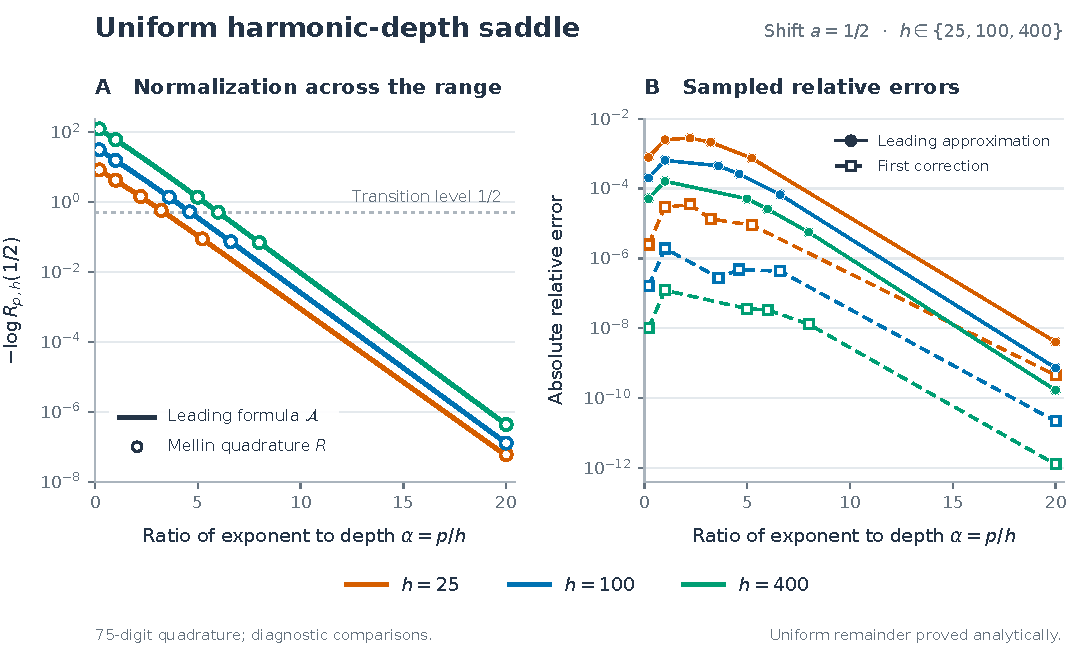
\includegraphics[width=\textwidth]{figures/uniform_harmonic_saddle.pdf}
\caption{Uniform harmonic-depth approximation at $a=1/2$, for
$h=25,100,400$. Both vertical axes are logarithmic.
\textbf{(A)} Solid curves show $-\log\mathcal A$ from the explicit
moving-saddle formula over $0.2\leq\alpha=p/h\leq20$; circles show
$-\log R$ from $75$-digit Mellin quadrature. The horizontal guide at
$1/2$ is the transition limit $-\log R_{h\log h,h}(1/2)\to1/2$.
\textbf{(B)} Absolute relative errors of the leading approximation
$\mathcal A$ and its first correction $\mathcal A(1+d_1/p)$ at the
$18$ sampled parameters. Connecting segments guide the eye.
These are numerical diagnostics; the analytic proof of
Theorem~\ref{cont26:thm:uniform} supplies the uniform remainder estimate.}
\label{cont26:fig:uniform-harmonic-saddle}
\end{figure}

\subsection{A uniform Laplace lemma and proof}
Put $y=xu$ in \eqref{cont26:eq:positive}. The phase and amplitude, normalized
at their unique saddle $u=1$, are
\begin{align}
 \phi(u)&=\log u-u+1+\frac{\theta}{x}
       \{H(xu)-H(x)-xH'(x)(u-1)\},\label{cont26:eq:phase}\\
 g_x(u)&=\frac1{u(1+e^{-xu})}.\label{cont26:eq:amp}
\end{align}
Thus $\phi(1)=\phi'(1)=0$, $-\phi''(1)=B$, and the exact integral is
\begin{equation}\label{cont26:eq:exact-scaled}
 R_{p,h}(a)=\frac{(h+a)^p x^p L(x)^h e^{-ax}}{\Gamma(p)}
             \int_0^\infty e^{p\phi(u)}g_x(u)\,du.
\end{equation}

The following four bounds hold uniformly in $x>0$ and
$0\leq\theta\leq1/w(x)$, a set containing every saddle parameter above.
\begin{enumerate}
\item Concavity of $H$ gives the global bound
\begin{equation}\label{cont26:eq:global-gamma-bound}
 \phi(u)\leq\log u-u+1\quad (u>0).
\end{equation}
\item The curvature is uniformly nondegenerate:
$1\leq B\leq1+w_0^{-1}\sup_{x>0}xw'(x)<\infty$.
\item On $1/2\leq u\leq3/2$, each fixed derivative of $\phi$ is
uniformly bounded. For $m\geq2$ the only extra term beyond a derivative
of $\log u-u+1$ is
$\theta x^{m-1}H^{(m)}(xu)$. Its boundedness follows from smoothness
at zero and exponential decay at infinity. Derivatives of $g_x$ are
uniformly bounded on the same interval, while
$1/2\leq g_x(1)\leq1$.
\item Globally $0<g_x(u)\leq1/u$.
\end{enumerate}

For completeness, these bounds suffice for a parameter-uniform Laplace
expansion, rather than merely a pointwise use of the method
\cite{DLMF23,TemmeUniform}. Choose a fixed $0<\eta<1/2$.
The contribution of $|u-1|\geq\eta$ is bounded by
\[
 \int_{|u-1|\geq\eta}\frac{e^{p(\log u-u+1)}}u\,du
 \leq C p^{-1/2}e^{-c_\eta p}.
\]
One direct proof divides the integral by
$e^p\Gamma(p)/p^p$ and applies the elementary exponential Markov
bound to a gamma random variable of shape $p$ and rate $p$.
The two tail exponents are
$1\pm\eta-1-\log(1\pm\eta)>0$.
This controls the unbounded domain and the singular factor $1/u$ at once.

On $|u-1|<\eta$, set $u=1+z/\sqrt p$. Taylor-expand the phase and
amplitude to a fixed order. Uniform derivative bounds give uniform
Taylor remainders. The inequality \eqref{cont26:eq:global-gamma-bound} supplies
a fixed Gaussian majorant in this neighborhood. Splitting further at
$|z|=p^\varepsilon$, with a sufficiently small fixed $\varepsilon>0$
for the chosen order, justifies expansion of the exponential with an
integrable polynomial-times-Gaussian remainder. Outside that smaller
interval the same majorant is smaller than every inverse power of $p$.
Odd powers integrate to zero on the symmetric neighborhood, and extending
each polynomial Gaussian integral to the whole real line changes it by
an exponentially small quantity. Expanding two additional orders when
necessary gives, for every fixed $J$,
\begin{equation}\label{cont26:eq:uniform-laplace}
 \int_0^\infty e^{p\phi(u)}g_x(u)\,du
 =g_x(1)\sqrt{\frac{2\pi}{pB}}
   \left\{\sum_{j=0}^J\frac{c_j(x,\theta)}{p^j}
                  +O_J(p^{-J-1})\right\}.
\end{equation}
Every division here is by a quantity uniformly bounded away from zero.
This also proves uniform boundedness of each $c_j$.

Let
$\Gamma^*(p)=\Gamma(p)/(\sqrt{2\pi}p^{p-1/2}e^{-p})$.
Substitution of \eqref{cont26:eq:uniform-laplace} into
\eqref{cont26:eq:exact-scaled} gives $\mathcal A/\Gamma^*(p)$ times the
bracketed expansion. The ordinary positive-real Stirling expansion,
with its remainder \cite{DLMF511}, now proves
Theorem~\ref{cont26:thm:uniform} by multiplication of two finite expansions.
The displayed $c_1=d_1+1/12$ is obtained from the Gaussian moments of
degrees two, four and six. This proves \eqref{cont26:eq:d1} as well.

\subsection{A finite coefficient compiler}
The proof specifies every coefficient without fitting any data. Let
$\phi_m=\phi^{(m)}(1)$ and $g_m=g_x^{(m)}(1)$.
For $j\geq0$ define the polynomial
\begin{equation}\label{cont26:eq:cj-polynomial}
 P_j(z)=[t^{2j}]
 \left(\sum_{r=0}^{2j}\frac{g_rz^rt^r}{r!}\right)
 \exp\left(\sum_{m=3}^{2j+2}\frac{\phi_mz^mt^{m-2}}{m!}\right).
\end{equation}
With the convention that odd Gaussian moments vanish,
\begin{equation}\label{cont26:eq:cj}
 c_j=\frac1{g_0}\sqrt{\frac B{2\pi}}
      \int_{\mathbb R}e^{-Bz^2/2}P_j(z)\,dz.
\end{equation}
The even moments are $(2r-1)!!B^{-r}$ after normalization.
Finally, as a formal power-series prescription,
\begin{equation}\label{cont26:eq:dj}
 \sum_{j\geq0}d_j\varepsilon^j
 =\exp\left(-\sum_{r\geq1}
 \frac{B_{2r}\varepsilon^{2r-1}}{2r(2r-1)}\right)
     \sum_{j\geq0}c_j\varepsilon^j.
\end{equation}
Only finitely many terms enter each coefficient. The expansion is an
asymptotic expansion; no convergence of \eqref{cont26:eq:dj} is asserted.

\subsection{Recovery of existing regimes and a new uniform connection}
For $a$ fixed and $p=\alpha h$ with $\alpha$ in a positive compact
interval, the new saddle solves
$x(w(x)+a/h)=\alpha$. Let $x_\alpha w(x_\alpha)=\alpha$ be the
source saddle. The implicit function theorem gives
\[
 x=x_\alpha-\frac{a x_\alpha}{h\{w(x_\alpha)+x_\alpha w'(x_\alpha)\}}
 +O(h^{-2}).
\]
The envelope derivative in $a/h$, or direct substitution, then gives
\begin{equation}\label{cont26:eq:old-recovery}
 \mathcal A(p,h,a)
 =C(\alpha,a)e^{-hI(\alpha)}(1+O(h^{-1})),
\end{equation}
where the source functions are
\[
 I(\alpha)=-\alpha\log(x_\alpha/\alpha)-\alpha-\log L(x_\alpha),
 \quad
 C(\alpha,a)=
 \frac{\sqrt{\alpha}}{\sqrt{\alpha+x_\alpha^2w'(x_\alpha)}}
 \frac{e^{a(\alpha-x_\alpha)}}{1+e^{-x_\alpha}}.
\]
The new result retains the actual saddle and therefore does not
expand a term whose error would grow with $\alpha$.

At the transition $p=h(\log h+c)$, $a,c$ in fixed compact sets,
write $\alpha=\log h+c$ and $\lambda=e^{-c}/2$.
Since $w(x)=1-e^{-x}/2+O(e^{-2x})$, the saddle has
$x=\alpha+O(\alpha/h)$, and consequently
\[
 hH(x)=-\lambda+O(\alpha/h),\qquad
 p\{\log(1+\delta)-\delta\}=O(\alpha/h),\qquad
 B=1+O(\alpha/h).
\]
It follows from the uniform theorem that
\[
 R_{p,h}(a)=e^{-\lambda}\{1+O(\alpha/h)\}.
\]
The source already proves a sharper transition expansion; the new
contribution is that the same unexpanded $\mathcal A$ has a uniform
relative error $O(1/p)$ across this transition and all intervening
values of $p/h$. Including $d_1/p$ improves it to $O(p^{-2})$.

For any fixed $\alpha_0>0$ and any function $M(h)\geq\alpha_0$,
Theorem~\ref{cont26:thm:uniform} gives, without an upper growth condition,
\begin{equation}\label{cont26:eq:expanding-range}
 \sup_{\substack{\alpha_0\leq p/h\leq M(h)\\a>0}}
 \left|\frac{R_{p,h}(a)}{\mathcal A(p,h,a)}-1\right|=O(h^{-1}).
\end{equation}
The corrected supremum is $O(h^{-2})$. This explicitly resolves the
expanding-range question in the proportional-depth chapter.

At $x\to\infty$, the phase tends to $\log u-u+1$, the amplitude
tends to $1/u$, and all $d_j$ for $j\geq1$ tend to zero. Thus the
gamma normalization is consistent with first-term dominance when also
$h e^{-x}\to0$, as happens for fixed $h$. The limit $x\to\infty$
alone does not imply $R\to1$ when the depth varies. Conversely,
the theorem also allows $p/h\to0$ provided $p\to\infty$; it makes
no claim about a bounded $p$, where a different endpoint expansion is
appropriate.

\subsection{Exact monotonicities}
The same positive representation gives useful checks on numerical work.
If $Y$ is gamma with shape $p$ and rate $h+a$, then
\[
 R_{p,h}(a)=\mathbb E\,k_h(Y),\qquad
 k_h(y)=\frac{(e^yL(y))^h}{1+e^{-y}}.
\]
The function $k_h$ is strictly increasing in $y$ and strictly decreasing
in $h$. Coupling gamma variables by addition proves that $R$ is strictly
increasing in $p$. Scaling a common gamma variable proves strict decrease
in $a$, and jointly increasing the rate and decreasing the kernel proves
strict decrease in the integer $h$ for fixed $p,a$. Also $0<R<1$.
These are exact statements, independent of an asymptotic regime.



\section{Joint asymptotics for reflected log-gamma moments}
\label{cont26:joint:sec:main}

Let
\[
 f(x)=\log\Gamma(x),\qquad B(x)=f(1-x),\qquad
 M_{n,m}=\int_0^1 f(x)^n B(x)^m\,dx.
\]
These mixed integrals are classical; they occur as $T_{n+m,n}$ in
\cite[Section~5]{ACEMKM}.  The fixed-$m$ expansions in the
repository do not give relative estimates when both exponents grow.
This section treats two parts of that unresolved regime.  First, a
global uniqueness theorem gives a full saddle expansion whenever
$m/n$ remains in a compact subset of $(0,\infty)$.  Second, an entirely
analytic transition theorem determines exactly how the leading
fixed-$m$ approximation fails near $n/(m+1)=\log m+O(1)$.
The first result uses a short, reproducible rational certificate for a
special-function inequality.  The transition theorem does not depend
on that certificate.

All exponents in this section may be positive real numbers; the
factorial $n!$ is then written $\Gamma(n+1)$.  The familiar inequalities
$0<f(x)\le-\log x$ on $(0,1)$ follow from $\psi(1)=-\gamma<0$,
$\psi'(x)>0$, and log-convexity of $\Gamma$ between $1$ and $2$.
The Taylor series and polygamma formulas used below are classical
\cite{DLMFTaylor,DLMFPolygamma}.

\subsection{A strict monotonicity theorem and one saddle for every ratio}

Define positive functions
\begin{equation}\label{cont26:joint:eq:hQ}
 h(x)=\frac{-\psi(x)}{\log\Gamma(x)},\qquad
 Q(x)=\frac{h(x)}{h(1-x)},\qquad 0<x<1.
\end{equation}
Direct differentiation gives
\begin{align}\label{cont26:joint:eq:D}
 D(x):=\frac{d}{dx}\log Q(x)
 ={}&\frac{-\psi(x)}{f(x)}+
     \frac{-\psi(1-x)}{f(1-x)}\notag\\
 &-\frac{\psi'(x)}{-\psi(x)}-
     \frac{\psi'(1-x)}{-\psi(1-x)}.
\end{align}

\begin{theorem}[Strict reflected elasticity inequality]
\label{cont26:joint:thm:Q}
For every $0<x<1$, $D(x)>0$.  Consequently $Q$ is a strictly increasing
real-analytic bijection from $(0,1)$ onto $(0,\infty)$, and
$Q(1-x)=Q(x)^{-1}$.  In particular,
\begin{equation}\label{cont26:joint:eq:product}
 \log\Gamma(x)\log\Gamma(1-x)
 \le \frac{\log^2\pi}{4},
\end{equation}
with equality exactly at $x=1/2$.
\end{theorem}

\begin{proof}
The identity $D(1-x)=D(x)$ reduces the problem to $0<x\le1/2$.
We first give an analytic proof on $0<x\le1/16$, and then describe the
finite rational certificate for $1/16\le x\le1/2$.

Write $L=-\log x$, $p=-\psi(x)$, $s=-\psi(1-x)$, and
$b=B(x)/x$.  The positive series
\[
 B(x)=\gamma x+\sum_{k\ge2}\frac{\zeta(k)}k x^k
\]
implies $s/b\ge1$ and $s\ge\gamma>1/2$.
Concavity of $\psi$ gives
$\psi(1+x)\le-\gamma+\zeta(2)x<0$ on this interval.
Thus $xp=1-x\psi(1+x)\ge1$, and $f(x)\le L$ gives
$xp/f(x)\ge1/L$.  The polygamma series yield
\[
 x^2\psi'(x)=1+x^2\psi'(1+x)\le1+2x^2,
 \qquad \psi'(1-x)\le\frac{\zeta(2)}{(1-x)^2}
 <\frac2{(1-x)^2}.
\]
Inserting these inequalities into \eqref{cont26:joint:eq:D} gives
\begin{equation}\label{cont26:joint:eq:endpoint-D}
 xD(x)\ge\frac1L-2x^2-\frac{4x}{(1-x)^2}>0.
\end{equation}
For the last inequality, $xL$ and $x^2L$ increase on $(0,1/16]$,
and $\log16<3$.  Therefore
\[
 L\left(2x^2+\frac{4x}{(1-x)^2}\right)
 \le\log16\left(\frac1{128}+\frac{64}{225}\right)
 <\frac{25251}{28800}<1.
\]

For the remaining compact interval, set
\[
 p_1=-\psi(x),\quad p_2=-\psi(1-x),\quad
 v_1=\psi'(x),\quad v_2=\psi'(1-x),\quad f_1=f(x),\quad f_2=B(x).
\]
The functions $f_1,p_1,v_1$ decrease, and $f_2,p_2,v_2$ increase.
If $a\le x\le b$, interval enclosures at the two endpoints therefore give
the rigorous rational lower bound
\begin{equation}\label{cont26:joint:eq:certificate-lower}
 D(x)\ge
 \frac{\underline p_1(b)}{\overline f_1(a)}
 +\frac{\underline p_2(a)}{\overline f_2(b)}
 -\frac{\overline v_1(a)}{\underline p_1(b)}
 -\frac{\overline v_2(b)}{\underline p_2(a)}.
\end{equation}
All denominators are positive.  Use the 112 intervals
$[j/256,(j+1)/256]$, $16\le j<128$, and the explicit enclosures in
Subsection~\ref{cont26:joint:subsec:certificate}.  Exact rational evaluation of
\eqref{cont26:joint:eq:certificate-lower}, reproduced by
\texttt{certify\_gamma\_saddle.py}, proves on every interval that
\begin{equation}\label{cont26:joint:eq:certificate-margin}
 D(x)\ge \frac{1693471917}{10^9}>0.
\end{equation}
The complete list of rational lower bounds is stored in
\texttt{gamma\_saddle\_certificate.json}.  Neither special-function
floating-point evaluations nor numerical differentiation enter these
checks.  This finite certificate completes the inequality on $(0,1)$.

Finally, $f(x)\sim-\log x$, $-\psi(x)\sim1/x$, and
$f(1-x)\sim\gamma x$ as $x\downarrow0$, so
$Q(x)\sim1/\log(1/x)\to0$.  Reflection gives the limit $+\infty$ at
one.  The derivative of the logarithm of the product in
\eqref{cont26:joint:eq:product} is $h(1-x)(1-Q(x))$.
Its unique zero is $x=1/2$, with positive derivative sign before that
point and negative sign afterward.  Since $\Gamma(1/2)=\sqrt\pi$,
the sharp bound and equality case follow.
\end{proof}

\begin{theorem}[Uniform joint saddle expansion]
\label{cont26:joint:thm:laplace}
Let $\lambda=m/n$ remain in a fixed compact subset $K\subset(0,\infty)$
as $n\to\infty$.  Let $x_\lambda$ be the unique solution of
\begin{equation}\label{cont26:joint:eq:saddle}
 Q(x_\lambda)=\lambda,
\end{equation}
and define
\[
 \Phi_\lambda(x)=\log f(x)+\lambda\log f(1-x),\qquad
 \kappa_\lambda=-\Phi_\lambda''(x_\lambda)>0.
\]
Then, uniformly for $\lambda\in K$,
\begin{align}\label{cont26:joint:eq:laplace}
 M_{n,m}={}&f(x_\lambda)^n f(1-x_\lambda)^m
 \sqrt{\frac{2\pi}{n\kappa_\lambda}}
 \left(1+\frac{C_1(\lambda)}n+O_K(n^{-2})\right),\\
 C_1(\lambda)={}&
 \frac{\Phi_\lambda^{(4)}(x_\lambda)}{8\kappa_\lambda^2}
 +\frac{5\Phi_\lambda^{(3)}(x_\lambda)^2}{24\kappa_\lambda^3}.
 \label{cont26:joint:eq:C1}
\end{align}
There is a full uniform expansion in integer powers of $1/n$.
Moreover $x_\lambda$ increases analytically from zero to one as
$\lambda$ increases from zero to infinity, and
$x_{1/\lambda}=1-x_\lambda$.
\end{theorem}

\begin{proof}
By \eqref{cont26:joint:eq:hQ},
\[
 \Phi_\lambda'(x)=h(1-x)(\lambda-Q(x)).
\]
Theorem~\ref{cont26:joint:thm:Q} proves that this is positive before
$x_\lambda$ and negative after it.  It also proves nondegeneracy:
\begin{equation}\label{cont26:joint:eq:curvature}
 \kappa_\lambda=h(1-x_\lambda)Q'(x_\lambda)>0.
\end{equation}
The analytic implicit-function theorem proves the assertions about
$x_\lambda$; reflection gives the last identity.

Compactness of $K$ keeps $x_\lambda$ a fixed distance from both
endpoints, and bounds $\kappa_\lambda$ away from zero.  All required
derivatives of the phase are then uniformly bounded in one fixed
neighborhood of the moving saddle.  The phase tends to $-\infty$
at either endpoint, uniformly for $\lambda\in K$: near zero it is
$\log\log(1/x)+\lambda\log x+O_K(1)$, and near one the analogous
formula follows by reflection.  Strict unimodality and compactness
give a uniform positive gap between the maximum and the phase
outside a fixed neighborhood of the saddle.  Thus the integral over
that complement is exponentially smaller than the saddle term.

In the neighborhood, put $u=\sqrt{n\kappa_\lambda}(x-x_\lambda)$
and Taylor-expand the analytic phase.  Gaussian domination justifies
termwise integration to every fixed order.  Odd powers integrate to
zero; the quartic term and the square of the cubic term give
\eqref{cont26:joint:eq:C1}.  To make the error assertion explicit, expand
through enough even orders on $|u|\le n^{1/10}$, use the uniform
Taylor remainder there, and bound its complement by
$O(e^{-c n^{1/5}})$.  This proves the stated relative error and full
uniform expansion without an unproved competing-saddle assumption.
\end{proof}

For reproducibility, the coefficient $C_j$ at arbitrary order can be
written as a finite sum.  All derivatives below are evaluated at
$x_\lambda$.  For nonnegative integers $r_3,\ldots,r_{2j+2}$ with
$\sum_{k=3}^{2j+2}(k-2)r_k=2j$, put
$R=\sum_{k=3}^{2j+2}k r_k$.  Then
\begin{equation}\label{cont26:joint:eq:allorders}
 C_j(\lambda)=
 \sum_{\sum(k-2)r_k=2j}
 \frac{(R-1)!!}{\kappa_\lambda^{R/2}}
 \prod_{k=3}^{2j+2}
 \frac1{r_k!}\left(\frac{\Phi_\lambda^{(k)}}{k!}\right)^{r_k},
\end{equation}
with $C_0=1$ and $(-1)!!=1$.  The constraint makes $R$ even.
This is simply coefficient extraction after expanding the exponential
of the terms of degree at least three in the local phase.

\begin{corollary}[Equal exponents]
\label{cont26:joint:cor:diagonal}
Set
\[
 a=\frac{\log\pi}{2},\qquad p=\gamma+2\log2,\qquad
 \kappa=\frac{2}{a^2}\left(p^2-\frac{\pi^2a}{2}\right).
\]
Then $\kappa>0$ and
\begin{equation}\label{cont26:joint:eq:diagonal}
 M_{n,n}=a^{2n}\sqrt{\frac{2\pi}{n\kappa}}
 \left(1+\frac{c_*}{n}+O(n^{-2})\right),
 \qquad c_*=-0.4398093541949199\ldots.
\end{equation}
The constant is exactly $c_*=\Phi_1^{(4)}(1/2)/(8\kappa^2)$, where
\begin{equation}\label{cont26:joint:eq:diagonal-fourth}
 \Phi_1^{(4)}(1/2)=2\left[
 \frac{\pi^4}{a}
 -\frac{56p\zeta(3)+3\pi^4/4}{a^2}
 +\frac{6p^2\pi^2}{a^3}
 -\frac{6p^4}{a^4}\right].
\end{equation}
Numerically $\kappa=6.2933987786891021\ldots$ and
$\sqrt{2\pi/\kappa}=0.9991882272949156\ldots$.
\end{corollary}
\begin{proof}
Here $x_1=1/2$ and all odd phase derivatives vanish.  Use
$\psi(1/2)=-p$, $\psi'(1/2)=\pi^2/2$,
$\psi''(1/2)=-14\zeta(3)$, and $\psi^{(3)}(1/2)=\pi^4$ in
Theorem~\ref{cont26:joint:thm:laplace}.  Differentiating $\log f$ four
times gives \eqref{cont26:joint:eq:diagonal-fourth}.
\end{proof}

\subsection{The compact interval certificate in full}
\label{cont26:joint:subsec:certificate}

This subsection specifies the arithmetic proof object independently
of any special-function library.  Every input is rational, and each
infinite tail has an explicit rational bound.

For $1\le z\le2$, put $y=(z-1)/(z+1)$ and use
\begin{equation}\label{cont26:joint:eq:log-bound}
 0\le\log z-2\sum_{r=0}^{31}\frac{y^{2r+1}}{2r+1}
 \le\frac{2y^{65}}{65(1-y^2)}.
\end{equation}
For any positive rational input, multiplication by an integral power
of two reduces its logarithm to this interval; $\log2$ is enclosed
by the same formula.  This controls all logarithms in the proof.

Euler's constant is enclosed with $N=32$ by
\begin{equation}\label{cont26:joint:eq:gamma-bound}
 H_N-\log N-\frac1{2N}<\gamma<
 H_N-\log N-\frac1{2N}+\frac1{12N^2}.
\end{equation}
For a short elementary verification, set
$e_N=H_N-\log N-1/(2N)$ and $z=1/(2N+1)$.
Expansion of $\log((1+z)/(1-z))$ gives
\[
 e_{N+1}-e_N=
 4\sum_{r\ge1}\frac{r}{2r+1}z^{2r+1}>0.
\]
The sequence $u_N=e_N+1/(12N^2)$ decreases, since
\[
 u_N-u_{N+1}=
 \sum_{r\ge1}\frac{8r(r-1)}{3(2r+1)}z^{2r+1}>0.
\]
Both sequences tend to $\gamma$, proving \eqref{cont26:joint:eq:gamma-bound}.
The certificate also verifies $1/2<\gamma<2/3$.
For each integer $k\ge2$, the elementary integral test gives
\begin{equation}\label{cont26:joint:eq:zeta-bound}
 \sum_{r=1}^{32}\frac1{r^k}+\frac{33^{1-k}}{k-1}
 \le\zeta(k)\le
 \sum_{r=1}^{32}\frac1{r^k}+\frac{32^{1-k}}{k-1}.
\end{equation}
In particular $1<\zeta(k)<2$.

For each grid endpoint $x\in[1/16,1/2]$, use the degree-40 series
\begin{align*}
 f_1(x)&=-\log x-\gamma x+
       \sum_{k=2}^{40}\frac{(-1)^k\zeta(k)}k x^k+\varepsilon_f,\\
 f_2(x)&=\gamma x+
       \sum_{k=2}^{40}\frac{\zeta(k)}k x^k+\varepsilon_B,\\
 p_1(x)&=x^{-1}+\gamma+
       \sum_{k=2}^{40}(-1)^{k+1}\zeta(k)x^{k-1}+\varepsilon_p,\\
 p_2(x)&=\gamma+
       \sum_{k=2}^{40}\zeta(k)x^{k-1}+\varepsilon_s,\\
 v_1(x)&=x^{-2}+
       \sum_{k=2}^{40}(-1)^k(k-1)\zeta(k)x^{k-2}+\varepsilon_v,\\
 v_2(x)&=\sum_{k=2}^{40}(k-1)\zeta(k)x^{k-2}+\varepsilon_u.
\end{align*}
With
\[
 E_f=\frac{2x^{41}}{41(1-x)},\qquad
 E_p=\frac{2x^{40}}{1-x},\qquad
 E_v=2x^{39}\left(\frac{40}{1-x}+\frac{x}{(1-x)^2}\right),
\]
one has $|\varepsilon_f|\le E_f$,
$|\varepsilon_p|\le E_p$, $|\varepsilon_v|\le E_v$,
and $0\le\varepsilon_B\le E_f$,
$0\le\varepsilon_s\le E_p$, $0\le\varepsilon_u\le E_v$.
These follow by bounding each omitted $\zeta(k)$ by two and summing
a geometric series or its derivative.

Substitute the rational intervals from
\eqref{cont26:joint:eq:log-bound}--\eqref{cont26:joint:eq:zeta-bound} with the correct
sign into these six formulas.  Evaluate
\eqref{cont26:joint:eq:certificate-lower} on the 112 adjacent intervals.
The smallest lower bound, rounded downward to denominator $10^9$,
is the number in \eqref{cont26:joint:eq:certificate-margin}; it occurs on
$[127/256,1/2]$.  This completely specifies the finite verification.
The following command replays all the fraction operations and compares
the stored proof object:
\begin{quote}\ttfamily
 python certify\_gamma\_saddle.py --check
\end{quote}
The script uses only the Python standard library and has no numerical
special-function dependency.  The role of the computation is the
finite family of strict rational inequalities, whose analytic coverage
has already been proved.  Replacing it by a short conceptual proof of
\eqref{cont26:joint:eq:D} is a useful further question.

\subsection{The small-ratio saddle has an exponential transseries}

The saddle approaches the endpoint on an exponential scale when
$\lambda\downarrow0$.  Define
\begin{equation}\label{cont26:joint:eq:cde}
 c=\frac{\zeta(2)}{2\gamma},\qquad d=c-\gamma,\qquad
 e=\gamma^2+\frac{\zeta(3)}{3\gamma}
                   -\frac{\zeta(2)^2}{8\gamma^2}.
\end{equation}
Here $d>0$: $\gamma<2/3$ and $\zeta(2)>1$ suffice.

\begin{proposition}[Endpoint location of the moving saddle]
\label{cont26:joint:prop:saddle-small}
As $\lambda\downarrow0$,
\begin{equation}\label{cont26:joint:eq:saddle-small}
 x_\lambda=e^{-1/\lambda}
 \left[1+\left(\frac d\lambda-\gamma\right)e^{-1/\lambda}
 +O\left(\lambda^{-2}e^{-2/\lambda}\right)\right].
\end{equation}
The corresponding expansion near $\lambda=\infty$ follows by reflection.
\end{proposition}
\begin{proof}
For $L=\log(1/x)\to\infty$, the convergent gamma series give
\[
 h(x)=\frac1{xL}\left[1+\gamma x+\frac{\gamma x}L+O(x^2)\right],
 \qquad h(1-x)=\frac1x[1+cx+O(x^2)].
\]
Consequently
\[
 Q(e^{-L})=\frac1L\left[1-de^{-L}
                      +\frac{\gamma e^{-L}}L+O(e^{-2L})\right].
\]
In the equation $Q(e^{-L})=\lambda$, first $L\sim1/\lambda$.
Writing $L=1/\lambda+\Delta$ and substituting once more gives
\[
 \Delta=\left(-\frac d\lambda+\gamma\right)e^{-1/\lambda}
          +O(\lambda^{-2}e^{-2/\lambda}).
\]
For instance, this error follows from the mean-value theorem applied
to $\lambda L-1+e^{-L}(d-\gamma/L)+O(e^{-2L})$, whose derivative
is $\lambda+O(e^{-L})$.  Exponentiating proves the proposition.
\end{proof}

\subsection{The critical window for the fixed-exponent approximation}

The leading fixed-$m$ estimate has the exact reference scale
\begin{equation}\label{cont26:joint:eq:reference}
 L_{n,m}=\frac{\gamma^m\Gamma(n+1)}{(m+1)^{n+1}}.
\end{equation}
Near the endpoint its underlying approximations are
$f(x)\simeq-\log x$ and $B(x)\simeq\gamma x$.
When $m$ grows, the relative corrections to these approximations
accumulate.  The transition studied below is governed by
$m\exp(-n/(m+1))$, not just by $m/n$.

\begin{theorem}[Critical-window transition with its first correction]
\label{cont26:joint:thm:critical}
Let $m\to\infty$, put
\[
 t=\frac n{m+1},\qquad \tau=m e^{-t},
\]
and suppose $t-\log m$ lies in a fixed bounded interval.
With $c,d,e$ from \eqref{cont26:joint:eq:cde}, uniformly in that interval,
\begin{equation}\label{cont26:joint:eq:critical}
 \frac{M_{n,m}}{L_{n,m}}
 =e^{d\tau}\left[
 1+\frac1m\left\{
 \frac t2(d\tau+d^2\tau^2)-(c+\gamma)\tau+e\tau^2
 \right\}
 +O\left(\frac{(\log m)^2}{m^2}\right)\right].
\end{equation}
In particular, if $n/(m+1)-\log m\to s\in\mathbb R$, then
\begin{equation}\label{cont26:joint:eq:critical-limit}
 \frac{M_{n,m}}{\gamma^m\Gamma(n+1)/(m+1)^{n+1}}
 \longrightarrow \exp(d e^{-s}).
\end{equation}
Thus the leading fixed-$m$ approximation has a nonvanishing relative
error throughout this window.  At $s=0$ the limiting ratio is
$e^d=2.334\ldots$.
\end{theorem}

\begin{proof}
Put $r=m+1$, and let $T$ have gamma density
\[
 \frac{r^{n+1}}{\Gamma(n+1)}T^n e^{-rT},\qquad T>0.
\]
The substitution $x=e^{-T}$ gives the exact expectation identity
\begin{equation}\label{cont26:joint:eq:gamma-expectation}
 \frac{M_{n,m}}{L_{n,m}}=\mathbb E Z(T),\qquad
 Z(T)=\left(\frac{f(e^{-T})}{T}\right)^n
       \left(\frac{B(e^{-T})}{\gamma e^{-T}}\right)^m.
\end{equation}
Since $t-\log m$ is bounded, $t\asymp\log m$ and $\tau$ stays in
a compact subinterval of $(0,\infty)$.

We first control the tails of the actual integrand.  There is a
constant $A>0$ such that
\[
 \log\frac{B(x)}{\gamma x}\le Ax\qquad(0<x\le1/2),
\]
because the quotient is analytic and equals one at zero.
Also $f(x)/(-\log x)\le1$.
For $T\ge t/2$, these facts give
$Z(T)\le\exp(A m e^{-T})\le\exp(C\sqrt m)$.
Gamma Chernoff bounds imply, for some $c_0>0$,
\[
 \mathbb P(|T-t|>1/2)\le
 \exp\left(-c_0\frac m{\log m}\right)
\]
for sufficiently large $m$; the shift between the mean and $t$ is
$1/r$.  Hence the contribution with $T\ge t/2$ and $|T-t|>1/2$
is smaller than every negative power of $m$.
For $\log2\le T<t/2$, the bound
$Z(T)\le\exp(A m/2)$ and the fixed-fraction lower-tail bound
$\mathbb P(T<t/2)\le\exp(-c_1 n)$ give the same conclusion,
since $n\asymp m\log m$.

The remaining interval $0<T<\log2$ is estimated before normalization.
It corresponds to $x>1/2$.  Positivity of the Taylor coefficients of
$B$ shows that $B(y)/y$ increases on $[0,1/2]$, so
\[
 f(x)\le(\log\pi)(1-x),\qquad
 f(1-x)\le-\log(1-x)\qquad(x\ge1/2).
\]
Thus the integral over this interval is at most
\begin{equation}\label{cont26:joint:eq:opposite-tail}
 (\log\pi)^n\int_0^{1/2}y^n(-\log y)^m\,dy
 \le\frac{(\log\pi)^n\Gamma(m+1)}{(n+1)^{m+1}}.
\end{equation}
After division by $L_{n,m}$, Stirling's formula gives logarithm
$-n\log(n/m)+O(n+m\log(n/m))$.
Here $n/m\asymp\log m$, so this is
$-n\log\log m+O(n)$ and tends to $-\infty$ faster than
any multiple of $\log m$.  This controls both endpoints and
justifies using a local expectation expansion on $|T-t|\le1/2$.
The Chernoff estimates also make the omitted tails of any fixed
polynomial in $T-t$ smaller than every negative power of $m$;
this follows either by a slightly smaller Chernoff exponent or by
Cauchy--Schwarz and the gamma moments.

For that expansion write $V=T-t$ and $H(T)=\log Z(T)$.
The convergent Taylor series at $x=0$ give
\begin{align*}
 \log\frac{B(x)}{\gamma x}
 &=cx+\left(\frac{\zeta(3)}{3\gamma}-\frac{c^2}{2}\right)x^2
   +O(x^3),\\
 \log\frac{f(x)}{-\log x}
 &=-\frac{\gamma x}{T}
 +\left(\frac{\zeta(2)}{2T}-\frac{\gamma^2}{2T^2}\right)x^2
 +O(x^3/T),\qquad x=e^{-T}.
\end{align*}
These estimates and their first four $T$-derivatives are uniform
on $|T-t|\le1/2$, since there $x\asymp1/m$ and $T\asymp\log m$.
Define
\[
 b_2=\frac{\zeta(3)}{3\gamma}-\frac{c^2}{2}.
\]
At $T=t$ they imply
\begin{align}
 H(t)&=d\tau+\frac1m\left[
 -\gamma\tau+\tau^2\left(b_2+\frac{\zeta(2)}2
                         -\frac{\gamma^2}{2t}\right)\right]
 +O(m^{-2}),\label{cont26:joint:eq:H0}\\
 H'(t)&=\tau\left(-d+\frac\gamma t\right)+O(m^{-1}),\notag\\
 H''(t)&=\tau\left(d-\frac{2\gamma}t-
                           \frac{2\gamma}{t^2}\right)+O(m^{-1}).\notag
\end{align}
The first four derivatives of $Z=e^H$ are bounded uniformly on the
local interval.  The exact gamma moments about $t=n/r$ are
\begin{align*}
 \mathbb EV&=r^{-1},\qquad
 \mathbb EV^2=t/r+2/r^2,\\
 \mathbb EV^3&=5t/r^2+6/r^3,\qquad
 \mathbb EV^4=3t^2/r^2+26t/r^3+24/r^4.
\end{align*}
Taylor-expand $Z(t+V)$ through degree three and use the fourth
absolute moment for the remainder.  The signed cubic moment is
$O(t/m^2)$; using an absolute cubic estimate would lose the claimed
order.  The tail bounds already proved permit replacement of
the local moments by the complete moments.  Therefore
\begin{equation}\label{cont26:joint:eq:expect-expansion}
 \mathbb E Z(T)=e^{H(t)}
 \left[1+\frac{H'(t)}m+
 \frac{t}{2m}\bigl(H''(t)+H'(t)^2\bigr)
 +O(t^2/m^2)\right].
\end{equation}
Insert \eqref{cont26:joint:eq:H0}.  All terms containing $1/t$ cancel.
The terms linear in $\tau$ reduce to
$td\tau/2-(c+\gamma)\tau$, and the quadratic terms reduce to
$td^2\tau^2/2+(b_2+\gamma^2)\tau^2$.
Since $b_2+\gamma^2=e$, this is \eqref{cont26:joint:eq:critical}.
The limit follows because $t/m\to0$ and $\tau\to e^{-s}$.
\end{proof}

The transition condition is approximately
$m\log m\asymp n$, more precisely $n=(m+1)(\log m+s)$.
The equality $m\log m=n$ has solution $m=n/W(n)$, so the nontrivial
transition exhibited by the theorem lies on an $n/W(n)$ scale.
This statement identifies the scale; the theorem
uses the exact variables $t$ and $\tau$, avoiding an error from
replacing $m+1$ by $m$ prematurely.

\subsection{Numerical checks and scope}

The script \texttt{check\_gamma\_joint\_asymptotics.py} uses
65-digit quadrature and numerical differentiation solely as
diagnostics.  Its data are in \texttt{gamma\_joint\_diagnostics.json}.
For equal exponents $n=20,40,80$, the relative errors of the
leading formula in \eqref{cont26:joint:eq:diagonal} are approximately
$2.20\cdot10^{-2}$, $1.10\cdot10^{-2}$, and $5.50\cdot10^{-3}$;
after including $c_*/n$, they become
$-4.76\cdot10^{-4}$, $-1.17\cdot10^{-4}$, and $-2.90\cdot10^{-5}$.
This is consistent with the proved first and second orders.

In the critical window with $s\approx0$, choosing $m=100,400,1600$
gives $n=465,2403,11812$.  The relative errors of $e^{d\tau}$ are
approximately $-1.67\cdot10^{-2}$, $-6.81\cdot10^{-3}$, and
$-2.37\cdot10^{-3}$.  Including the displayed correction reduces
them to $-7.89\cdot10^{-4}$, $-1.08\cdot10^{-4}$, and
$-1.24\cdot10^{-5}$, respectively.  These values are not interval
certificates; the analytic proof supplies the asymptotic statements.

The two proved joint regimes do not constitute one expansion uniform
over all exponent ratios. Section~\ref{cont26:sec:further} specifies the
remaining matching, coefficient, and optimal-truncation questions.

\begin{figure}[tbp]
\centering
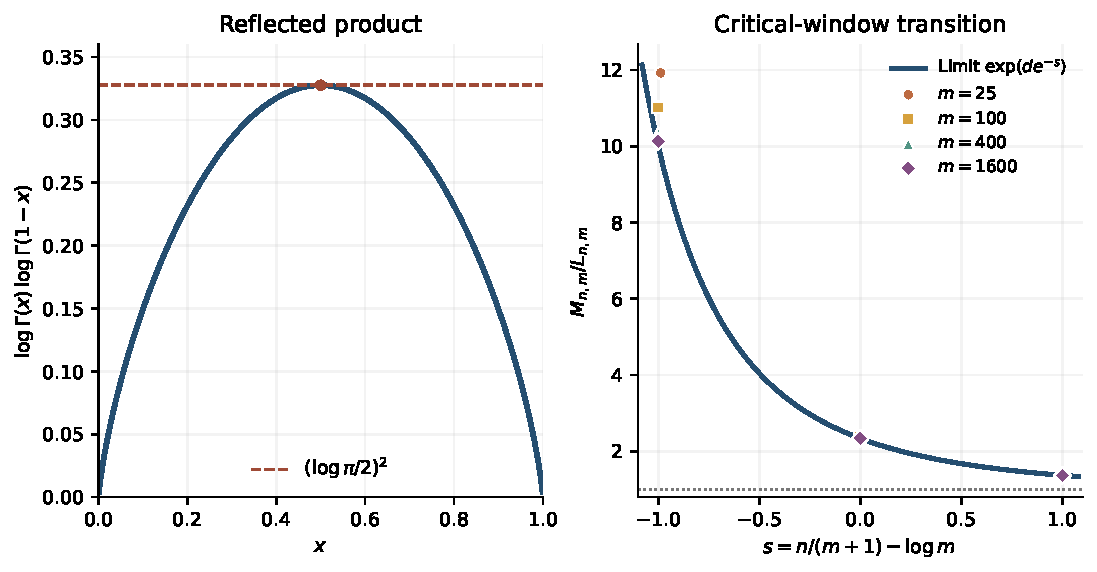
\includegraphics[width=\textwidth]{figures/gamma_joint.pdf}
\caption{Left: the reflected product and its sharp maximum. Right: the
critical-window profile $\exp(d e^{-s})$ with numerical quadrature
for $m=25,100,400,1600$. The horizontal dotted line is the fixed-$m$
leading reference ratio one. The analytic theorem proves the profile;
the plotted points are numerical diagnostics.}
\label{cont26:fig:gamma-joint}
\end{figure}

\section{Lerch deformation: loss of real zeros and forced bifurcations}
\label{cont26:sec:lerch-bifurcations}

The manuscript proves eventual saturation of the positive-zero bound as
the parameter-derivative order grows, uniformly in the Lerch deformation
\cite{ProveIt}. At a fixed small derivative order the geometry is different.
We prove an exact count for sufficiently small positive deformation
parameters. Multiple elementary roots generally leave the real axis.
At indices three and four this forces an interior change in the number
of positive zeros before the Stieltjes endpoint is reached.

For integers $n\geq0$, $k\geq1$, let
\begin{equation}\label{cont26:eq:bif-family}
 f_{n,k}(a)=\frac{d^k}{da^k}\frac{\log^n a}{a},\qquad
 D_{n,k}^{\rho}(a)=\sum_{m=0}^{\infty}\rho^m f_{n,k}(a+m)
 \quad (a>0,\ 0\leq\rho\leq1).
\end{equation}
Here $0^0=1$ in the $m=0$ summand. The differentiated series is absolutely
convergent even at $\rho=1$, and
$D_{n,k}^{1}(a)=\gamma_n^{(k)}(a)$ for the Laurent convention
\[
 \zeta(s,a)=\frac1{s-1}
       +\sum_{n\geq0}\frac{(-1)^n}{n!}\gamma_n(a)(s-1)^n.
\]
For $\rho<1$, it equals $\partial_a^k\ell_n(\rho,a)$ with
$\ell_n(\rho,a)=\sum_{m\geq0}\rho^m\log^n(a+m)/(a+m)$.
In particular, these are order derivatives of the Lerch transcendent;
at $a=1$ their undeformed-in-$a$ antecedents specialize to order
derivatives of $\operatorname{Li}_s(\rho)$.

Define the rational polynomial
\begin{equation}\label{cont26:eq:bif-polynomial}
 P_{n,k}(x)=n![t^n]\left(e^{xt}\prod_{j=1}^k(1+t/j)\right).
\end{equation}
Coefficient extraction after differentiating $a^{-1-t}$ gives
\begin{equation}\label{cont26:eq:bif-elementary}
 (-1)^{n+k} f_{n,k}(a)=k!a^{-k-1}P_{n,k}(-\log a).
\end{equation}
The sign normalization
$F_{n,k}^{\rho}=(-1)^{n+k}D_{n,k}^{\rho}$ does not affect zeros.

\subsection{The elementary roots and uniform exclusion of escaping zeros}

\begin{lemma}\label{cont26:lem:bif-elementary-roots}
If $n>k\geq1$ and $d=n-k$, then $P_{n,k}$ has a root of multiplicity
$d$ at zero and precisely $k$ other roots, all simple and negative.
Its first nonzero coefficient is
\[
 [x^d]P_{n,k}(x)=\frac{n!}{d!\,k!}.
\]
\end{lemma}
\begin{proof}
The polynomial is $\prod_{j=1}^k(1+\partial_x/j)x^n$. If a polynomial
$p$ has real roots $r_i$ of multiplicities $m_i$, the new noninherited
roots of $p+c p'$ solve
\[
 \frac{p'(x)}{p(x)}=\sum_i\frac{m_i}{x-r_i}=-1/c.
\]
For $c>0$ the left side decreases strictly between its poles. There is
one new simple root in every intervening interval and one to the left
of all the old roots, and there is none to their right. Every inherited
multiple root loses one unit of multiplicity. Induction from $x^n$
therefore gives the asserted configuration. The coefficient follows
from the top coefficient $1/k!$ in $\prod_{j=1}^k(1+t/j)$.
\end{proof}

Let $A_{n,k}>1$ be the largest zero of $f_{n,k}$, equivalently the
exponential of the negative of the smallest root of $P_{n,k}$.

\begin{lemma}[No escape through either endpoint]\label{cont26:lem:bif-no-escape}
For fixed $n>k\geq1$ there is $\varepsilon_{n,k}>0$ such that every
positive zero of $D_{n,k}^{\rho}$, for every $\rho\in[0,1]$, lies in
$[\varepsilon_{n,k},A_{n,k}]$. For $\rho>0$ the upper inequality is strict.
Moreover $D_{n,k}^{\rho}\to f_{n,k}$ uniformly on every compact
subinterval of $(0,\infty)$ as $\rho\downarrow0$, including every fixed
number of $a$-derivatives.
\end{lemma}
\begin{proof}
The $m=0$ term in the normalized series satisfies
\[
 F_{n,k}^{0}(a)\sim k!a^{-k-1}\log^n(1/a)\longrightarrow+\infty
 \qquad(a\downarrow0).
\]
For $0<a\leq1$, the sum of the absolute values of all $m\geq1$ terms is
bounded independently of $\rho\in[0,1]$: each is bounded by a constant
times $(1+\log^n(m+1))/m^{k+1}$, whose series converges.
Thus the $m=0$ term dominates uniformly near zero.

For $a>A_{n,k}$, the argument $-\log(a+m)$ lies strictly to the left
of every root of $P_{n,k}$ for all $m\geq0$. Consequently all summands
have the same nonzero sign. At $a=A_{n,k}$ the $m=0$ summand vanishes
and the others have that common strict sign when $\rho>0$. This excludes
the upper endpoint and infinity. On a compact positive $a$-interval,
the same summable majorants, with $k$ increased for the derivatives,
give the final assertion by dominated convergence.
\end{proof}

\subsection{Complete small-parameter count and Puiseux branches}

\begin{theorem}[Unfolding the multiple elementary root]
\label{cont26:thm:bif-small-rho}
Fix $n>k\geq1$, put $d=n-k$, and define
\begin{equation}\label{cont26:eq:bif-constants}
 A=\frac{n!}{d!},\qquad
 B=\frac{k!}{2^{k+1}}P_{n,k}(-\log2).
\end{equation}
Assume $B\ne0$. For all sufficiently small $\rho>0$, every positive
zero of $D_{n,k}^{\rho}$ is simple and their exact number is
\begin{equation}\label{cont26:eq:bif-count}
 k+\begin{cases}
 1,&d\text{ odd},\\
 2,&d\text{ even and }B<0,\\
 0,&d\text{ even and }B>0.
 \end{cases}
\end{equation}
The $k$ zeros continuing the elementary zeros different from one are
real analytic functions of $\rho$. All $d$ complex zeros near $a=1$
are convergent Puiseux branches. Writing $t=\rho^{1/d}$ and letting
$y_1,\ldots,y_d$ be the distinct roots of
\begin{equation}\label{cont26:eq:bif-leading-equation}
 A y^d+B=0,
\end{equation}
these branches have the form
\begin{equation}\label{cont26:eq:bif-puiseux}
 a_j(\rho)=1-y_j\rho^{1/d}+O(\rho^{2/d}).
\end{equation}
Their series converge for sufficiently small $t$. In particular,
if $d\geq3$, the number in \eqref{cont26:eq:bif-count} is strictly less than $n$.
\end{theorem}
\begin{proof}
For $|\rho|<1$ the series is normally convergent on compact subsets
of $\Re a>0$ and hence jointly holomorphic in $(a,\rho)$. The principal
logarithm is unambiguous on this half-plane. The implicit-function
theorem continues each of the $k$ nonunit elementary zeros uniquely
and real analytically.

Near the remaining zero use the analytic coordinate $a=e^{-x}$.
Equations~\eqref{cont26:eq:bif-elementary} and \eqref{cont26:eq:bif-constants} give
\begin{equation}\label{cont26:eq:bif-local}
 F_{n,k}^{\rho}(e^{-x})
       =A x^d+B\rho+O(x^{d+1}+\rho x+\rho^2).
\end{equation}
Substitute $\rho=t^d$ and $x=ty$, divide by $t^d$, and extend
analytically to $t=0$. The resulting function equals $Ay^d+B$ at zero.
Its $d$ roots are simple because $AB\ne0$, so the implicit-function
theorem supplies $d$ analytic branches $y_j(t)=y_j+O(t)$. Rouch\'e's
theorem on a fixed small circle around $x=0$ shows that these exhaust
the zeros converging to zero. A branch is real for small positive $t$
exactly when its leading root $y_j$ is real: real leading roots continue
by conjugation and uniqueness; nonreal leading roots stay nonreal.
The polynomial $Ay^d+B$ has precisely the real-root count displayed
in \eqref{cont26:eq:bif-count}, since $A>0$.

Finally, Lemma~\ref{cont26:lem:bif-no-escape} confines every positive zero to
a fixed compact interval. Delete disjoint small neighborhoods of the
elementary zeros from that interval. The limit $f_{n,k}$ is bounded
away from zero on the remaining compact set; uniform convergence
excludes every additional zero there. Thus the local branch count is
the global positive-zero count. Simplicity follows from the nonzero
implicit derivatives, at both the ordinary and rescaled branches.
\end{proof}

The nonvanishing condition is displayed explicitly in the general
statement. For the following first-derivative specialization, its sign
and nonvanishing have an elementary proof for every index.

\begin{corollary}[All indices at first derivative order]
\label{cont26:cor:bif-kone}
For every fixed integer $n\geq2$, and all sufficiently small $\rho>0$,
$D_{n,1}^{\rho}$ has exactly one positive zero if $n$ is odd and
exactly two if $n$ is even. All are simple. One zero tends to $e^n$
and depends real analytically on $\rho$. When $n$ is even, the second
zero satisfies
\begin{equation}\label{cont26:eq:bif-even-root}
 a_{\mathrm{small}}(\rho)=1-\kappa_n\rho^{1/(n-1)}
             +O(\rho^{2/(n-1)}),\qquad
 \kappa_n=\log2\left(\frac{n-\log2}{4n}\right)^{1/(n-1)}>0.
\end{equation}
The root tending to $e^n$ moves initially to the left:
\begin{align}\label{cont26:eq:bif-large-root}
 a_{\mathrm{large}}(\rho)&=e^n-C_n\rho+O(\rho^2),\\
 C_n&=\frac{e^{3n}\log^{n-1}(e^n+1)
                    (\log(e^n+1)-n)}{n^{n-1}(e^n+1)^2}>0.\notag
\end{align}
\end{corollary}
\begin{proof}
Here
\[
 P_{n,1}(x)=x^{n-1}(x+n),\qquad
 f_{n,1}(a)=\frac{\log^{n-1}a\,(n-\log a)}{a^2}.
\]
Since $0<\log2<1<n$, the constant $B$ has sign $(-1)^{n-1}$.
For odd $n$ the multiplicity $n-1$ is even and $B>0$, giving no
real branch near one. For even $n$ it is odd and $B<0$, giving one
positive leading root $y=\kappa_n$ in \eqref{cont26:eq:bif-leading-equation}.
This proves the count and \eqref{cont26:eq:bif-even-root}.
At $a=e^n$,
$f'_{n,1}(e^n)=-n^{n-1}e^{-3n}$. Implicit differentiation of
$f_{n,1}(a)+\rho f_{n,1}(a+1)+O(\rho^2)=0$ gives
$a'(0)=-f_{n,1}(e^n+1)/f'_{n,1}(e^n)=-C_n$.
\end{proof}

For example, the double elementary zero for $n=3$ gives a conjugate
nonreal pair with
$a=1\mp i\kappa_3\sqrt\rho+O(\rho)$, whereas for $n=4$ the triple zero
gives one real branch below one and a nonreal conjugate pair. The
manuscript's eventual simplicity theorem is fully consistent with
this result: its derivative order tends to infinity, while the present
theorem fixes the derivative order and lets the deformation tend to zero.

\subsection{The logarithmic singularity at the Stieltjes endpoint}

An elementary tail calculation supplies a complementary expansion as
$\rho\uparrow1$. It gives the precise regularity that is not visible
in continuity of the positive-kernel representation. In this subsection
the indices are fixed and the limit concerns the deformation parameter.

For $0\leq j<k$ define the absolutely convergent moments
\begin{equation}\label{cont26:eq:bif-weighted-moments}
 M_{n,k,j}(a)=\sum_{m=0}^{\infty}m^j f_{n,k}(a+m),
 \qquad M_{n,k,0}(a)=\gamma_n^{(k)}(a).
\end{equation}
The $m=0$ factor is one when $j=0$ and zero otherwise.

\begin{theorem}[Endpoint expansion with its first nonanalytic term]
\label{cont26:thm:bif-rho-one}
Fix integers $n\geq0$, $k\geq1$ and a compact interval
$I\subset(0,\infty)$. Put $\epsilon=-\log\rho$ and
$L=\log(1/\epsilon)$. As $\epsilon\downarrow0$, uniformly for $a\in I$,
\begin{align}\label{cont26:eq:bif-rho-one}
 D_{n,k}^{e^{-\epsilon}}(a)
  ={}&\sum_{j=0}^{k-1}\frac{(-\epsilon)^j}{j!}M_{n,k,j}(a)
       +\frac{\epsilon^k L^{n+1}}{n+1}\\
     &\quad+O_{n,k,I}\bigl(\epsilon^k(1+L^n)\bigr).\notag
\end{align}
Thus the family is $C^{k-1}$ at the endpoint in the deformation
parameter, but its $k$th one-sided derivative is not finite there.
In particular it is not $C^k$. The coefficient of the leading
nonanalytic term is independent of $a$ and $k$.
\end{theorem}
\begin{proof}
For large $m$, uniformly on $I$, differentiation of
$\log^n(a+m)/(a+m)$ gives
\begin{equation}\label{cont26:eq:bif-large-m}
 f_{n,k}(a+m)=(-1)^k k!\frac{\log^n m}{m^{k+1}}+E_{n,k}(a,m).
\end{equation}
For $n\geq1$ the error is bounded by a constant times
\[
 \frac{1+\log^{n-1}m}{m^{k+1}}
       +\frac{1+\log^n m}{m^{k+2}};
\]
for $n=0$ it is $O(m^{-k-2})$. Indeed, the leading term arises when
all $k$ derivatives fall on $1/(a+m)$; every differentiation of a
logarithm lowers its degree, and replacement of $a+m$ by $m$ adds
one inverse power. This also proves convergence and local uniform
convergence of all the moments in \eqref{cont26:eq:bif-weighted-moments}.

Write
\[
 r_k(v)=e^{-v}-\sum_{j=0}^{k-1}\frac{(-v)^j}{j!}.
\]
Taylor's theorem and the finite polynomial bound give
\begin{align}\label{cont26:eq:bif-exponential-remainders}
 r_k(v)&=\frac{(-1)^k v^k}{k!}+O_k(v^{k+1})
                         &&(0\leq v\leq1),\\
 |r_k(v)|&\leq C_k v^{k-1}&&(v\geq1).\notag
\end{align}
Subtract the finite moment sum in \eqref{cont26:eq:bif-rho-one} from the
defining series. The remainder is exactly
$\sum_{m\geq1}f_{n,k}(a+m)r_k(\epsilon m)$.
Put $N=\lfloor1/\epsilon\rfloor$. In the range $m\leq N$ the error
from the first line of \eqref{cont26:eq:bif-exponential-remainders} is bounded by
\[
 C\epsilon^{k+1}\sum_{m\leq N}
                 m^{k+1}|f_{n,k}(a+m)|
   \leq C'\epsilon^k(1+L^n).
\]
Its retained part is
\[
 \frac{(-1)^k\epsilon^k}{k!}
       \sum_{m\leq N}m^k f_{n,k}(a+m).
\]
By \eqref{cont26:eq:bif-large-m}, ordinary integral comparison for logarithmic
harmonic sums gives
\[
 \sum_{m\leq N}m^k f_{n,k}(a+m)
   =(-1)^k k!\left\{\frac{L^{n+1}}{n+1}
                                +O(1+L^n)\right\}.
\]
For $n=0$ the error contributed by \eqref{cont26:eq:bif-large-m} is bounded;
for $n\geq1$ its lower logarithmic terms sum to $O(1+L^n)$.
The replacement of $\log N$ by $L$ is absorbed in the same error.
The two factors $(-1)^k$ cancel, producing the positive coefficient
in the theorem.

Finally the range $m>N$, using the second bound in
\eqref{cont26:eq:bif-exponential-remainders}, is at most
\[
 C\epsilon^{k-1}\sum_{m>N}\frac{1+\log^n m}{m^2}
       =O\bigl(\epsilon^k(1+L^n)\bigr).
\]
This proves the expansion with the claimed uniformity.

Differentiation with respect to $\epsilon$ through order $k-1$ is
justified at zero by the absolutely convergent weighted moment series,
uniformly on $I$. For clarity, the failure of the next derivative can
also be checked directly, without differentiating a big-$O$ term.
Put $G(\epsilon)=D_{n,k}^{e^{-\epsilon}}(a)$. Then
\[
 G^{(k-1)}(\epsilon)
   =(-1)^{k-1}\sum_{m\geq0}m^{k-1}e^{-\epsilon m}f_{n,k}(a+m).
\]
Apply the same split at $m=\lfloor1/\epsilon\rfloor$ to the difference
between this expression and its value at zero. Its summand has leading
coefficient $-k!\log^n m/m^2$, by \eqref{cont26:eq:bif-large-m}, and therefore
\[
 \frac{G^{(k-1)}(\epsilon)-G^{(k-1)}(0)}{\epsilon}
   =\frac{k!}{n+1}L^{n+1}+O(1+L^n)\longrightarrow+\infty.
\]
This proves the failure of a finite $k$th one-sided derivative. The
change of coordinates $\rho=e^{-\epsilon}$ is smooth with nonzero
derivative at zero; its lower-order chain-rule terms have finite limits.
Thus the same endpoint regularity holds in $\rho$.
\end{proof}

\begin{corollary}[Displacement of a simple Stieltjes zero]
\label{cont26:cor:bif-stieltjes-displacement}
Fix an integer $n\geq1$. Let $a_*>0$ be a simple zero of $\gamma_n'(a)$, so
$\gamma_n''(a_*)\ne0$. For $\rho<1$ sufficiently close to one there is a
unique nearby simple zero $a_*(\rho)$ of $D_{n,1}^{\rho}$. With
$\epsilon=-\log\rho$ and $L=\log(1/\epsilon)$,
\begin{equation}\label{cont26:eq:bif-root-displacement}
 a_*(\rho)=a_*
   -\frac{\epsilon L^{n+1}}{(n+1)\gamma_n''(a_*)}
   +O\bigl(\epsilon(1+L^n)\bigr).
\end{equation}
\end{corollary}
\begin{proof}
Local uniform convergence of the series and its $a$-derivative gives
a unique simple zero near $a_*$. The $k=1$ specialization of
Theorem~\ref{cont26:thm:bif-rho-one} is
\[
 D_{n,1}^{e^{-\epsilon}}(a)-\gamma_n'(a)
     =\frac{\epsilon L^{n+1}}{n+1}
           +O\bigl(\epsilon(1+L^n)\bigr),
\]
uniformly on a small interval around $a_*$. A derivative bounded away
from zero first gives $a_*(\rho)-a_*=O(\epsilon L^{n+1})$.
Taylor expansion of $\gamma_n'$ at $a_*$ then gives the displayed
formula. Its quadratic error is absorbed because
$\epsilon^2L^{2n+2}=o(\epsilon(1+L^n))$.
\end{proof}

The logarithmic enhancement means that a very small value of $1-\rho$
can still noticeably displace a fixed-index zero. This is a proved
endpoint scale. It does not determine where an interior multiple root
occurs, because the simple-root expansion ceases to apply when the
derivative in its denominator approaches zero.

\subsection{Fresh exact endpoint signs}

We recall, with proof, the global zero bound used to upgrade sign changes
to exact endpoint counts. It is the result entitled ``Global bound on
positive zeros'' in Chapter~10 of the source manuscript; the accompanying
results are entitled ``Strictly real-rooted reciprocal-gamma polynomials''
and ``Appell--Laplace representation'' \cite{ProveIt}.
Define reciprocal-gamma Appell polynomials $Q_n$ by
\[
 \frac{e^{xt}}{\Gamma(1+t)}=\sum_{n\geq0}Q_n(x)\frac{t^n}{n!}.
\]
\begin{lemma}[Global positive-zero bound]\label{cont26:lem:bif-global-count}
For every $n\geq0$, $k\geq1$, and $0\leq\rho\leq1$, the function
$D_{n,k}^{\rho}$ has at most $n$ positive zeros, counted with multiplicity.
\end{lemma}
\begin{proof}
The Weierstrass product is
\[
 \frac1{\Gamma(1+t)}=e^{\gamma t}
             \prod_{j\geq1}(1+t/j)e^{-t/j}.
\]
Taking $n![t^n]$ after multiplication by $e^{xt}$ turns finite products
into the operators $1+\partial_x/j$ and real translations applied to
$x^n$. These preserve real-rootedness by the operator proof in
Lemma~\ref{cont26:lem:bif-elementary-roots}. Local uniform convergence of the
product gives coefficient convergence of the resulting monic polynomials,
so the limiting $Q_n$ is real-rooted. For $n\geq1$, remove the first
$n-1$ factors before taking the limit. The remaining tail still gives
a real-rooted monic polynomial. Restoring the removed factors, including
their commuting real translations, applies $n-1$ root-preserving
operators, which reduce every inherited multiplicity until all roots
are simple. Thus $Q_n$ has exactly $n$ distinct real roots. For $n=0$
one has $Q_0=1$.

The Mellin integral gives the identity
\[
 \sum_{n\geq0}\frac{(-1)^{n+k}}{n!}D_{n,k}^{\rho}(a)t^n
   =\frac1{\Gamma(1+t)}\int_0^\infty
                   \frac{x^{k+t}e^{-ax}}{1-\rho e^{-x}}\,dx
\]
for $|t|<k$ in a neighborhood of zero. It follows either by
differentiating $(a+m)^{-1-t}$ $k$ times, or by canceling
$\Gamma(k+1+t)$ against its rising factorial. Coefficient comparison
proves
\begin{equation}\label{cont26:eq:bif-laplace}
 F_{n,k}^{\rho}(a)=\int_0^\infty
       \frac{x^ke^{-ax}}{1-\rho e^{-x}}Q_n(\log x)\,dx.
\end{equation}
At zero, $1/(1-\rho e^{-x})\leq1/(1-e^{-x})=O(x^{-1})$,
so $x^{k-1}|\log x|^n$ supplies an integrable majorant. At infinity
$e^{-ax}$ dominates all the logarithmic and polynomial factors.
These estimates justify coefficient extraction, differentiation in $a$,
and multiplication of the kernel by any fixed polynomial.

The signed kernel in \eqref{cont26:eq:bif-laplace} has exactly $n$ sign changes.
For completeness, let $G$ be a Laplace transform of such a kernel.
If there are no sign changes, $G$ has a fixed strict sign. Otherwise
choose one sign-change point $x_0$. Multiplication of the kernel by
$x_0-x$ removes that sign change and introduces none. Its transform is
$(\partial_a+x_0)G=e^{-x_0a}(e^{x_0a}G)'$ and, by induction, has at
most $n-1$ zeros counted with multiplicity and is not identically zero.
Therefore $G$ also cannot be identically zero. Any finite collection of
$M$ zeros of $G$, counted with multiplicity, forces at least $M-1$ zeros
of $(e^{x_0a}G)'$ by Rolle's theorem, including inherited multiplicities.
Hence $M\leq n$. The assertion holds for every finite collection and
therefore for all positive zeros, completing the induction and proof.
\end{proof}

The following are newly replayed rational enclosures for
\[
 V_n(a)=(-1)^{n+1}a^2\gamma_n'(a).
\]
Each displayed decimal endpoint is an exact terminating rational number.
\begin{center}
\begin{tabular}{cclc}
\hline
$n$&$a$&Interval containing $V_n(a)$&Sign\\
\hline
3&$4/5$&$[0.163799,\ 0.163919]$&$+$\\
3&$11/10$&$[-0.041066,\ -0.040839]$&$-$\\
3&$3/2$&$[0.055828,\ 0.056247]$&$+$\\
3&$21/10$&$[-0.245836,\ -0.245015]$&$-$\\
4&$4/5$&$[0.038668,\ 0.039282]$&$+$\\
4&$47/50$&$[-0.003812,\ -0.002965]$&$-$\\
4&$6/5$&$[0.021074,\ 0.022453]$&$+$\\
4&$17/10$&$[-0.037951,\ -0.035186]$&$-$\\
4&$11/5$&$[0.148603,\ 0.153231]$&$+$\\
\hline
\end{tabular}
\end{center}

For reproducibility, the included script uses only Python's standard
library and outward integer arithmetic on the grid $2^{-160}\mathbb Z$.
It sums the first $M=1000$ terms of \eqref{cont26:eq:bif-family} at $k=1,\rho=1$.
For a positive rational argument, power-of-two range reduction brings
the logarithm to $1\leq x\leq2$. With $u=(x-1)/(x+1)\in[0,1/3]$, it uses
\begin{equation}\label{cont26:eq:bif-log-certificate}
 0\leq\log x-2\sum_{j=0}^{J-1}\frac{u^{2j+1}}{2j+1}
 \leq\frac{2u^{2J+1}}{(2J+1)(1-u^2)},\qquad J=64.
\end{equation}
All powers, divisions and the geometric remainder are enclosed by
integer floor and ceiling. Inverting the argument handles logarithms
below one. Ordinary interval multiplication then evaluates $f_{n,1}$.

The tail needs only a monotone integral comparison. Put $b=a+M$ and
$h_n(x)=-f_{n,1}(x)$. For $n=3,4$ and $\log x\geq6$, this function is
positive and decreasing, since
\[
 h_n'(x)=-\frac{\log^{n-2}x}{x^3}
          \{2\log^2x-3n\log x+n(n-1)\}<0.
\]
Every argument $b$ above satisfies $\log b>6$. As
$\int_b^\infty h_n(x)\,dx=\log^n b/b$, one has the exact enclosure
\begin{equation}\label{cont26:eq:bif-tail-certificate}
 f_{n,1}(b)-\frac{\log^n b}{b}
 \leq\sum_{m=M}^{\infty}f_{n,1}(a+m)
 \leq-\frac{\log^n b}{b}.
\end{equation}
Combining these bounds proves every displayed sign; the JSON artifact
also contains the finer integer endpoints before decimal display rounding.
Thus these signs do not depend on quadrature or a special-function library.

\begin{corollary}[Forced interior multiple roots]
\label{cont26:cor:bif-interior}
For each $n\in\{3,4\}$ there are $\rho_*\in(0,1)$ and $a_*>0$ such that
\begin{equation}\label{cont26:eq:bif-discriminant}
 D_{n,1}^{\rho_*}(a_*)=0,
 \qquad \partial_aD_{n,1}^{\rho_*}(a_*)=0.
\end{equation}
At $\rho=1$ there are exactly $n$ positive zeros, all simple, and this
count persists for $\rho<1$ sufficiently close to one. For small positive
$\rho$ the counts are instead one and two, respectively.
\end{corollary}
\begin{proof}
The certified signs give $n$ disjoint intervals with sign changes.
The global bound with multiplicity shows that these are all the roots
and each is simple. Local uniform convergence as $\rho\uparrow1$ of the
series and its $a$-derivative preserves a unique simple root in each
small interval. The global bound excludes extras. The small-parameter
counts are Corollary~\ref{cont26:cor:bif-kone}.

If every root were simple throughout $0<\rho<1$, the implicit-function
theorem and compact exclusion of both endpoints would make the number
of positive roots locally constant on this connected interval, hence
constant. More explicitly, finitely many small root neighborhoods and
the zero-free compact complement yield a common parameter neighborhood
on which no root can be added or lost. The different endpoint counts
contradict constancy. Therefore \eqref{cont26:eq:bif-discriminant} holds at
an interior parameter.
\end{proof}

Ordinary numerical quadrature of \eqref{cont26:eq:bif-laplace}, followed by a
two-variable solve, suggests transitions near
\[
\begin{array}{c|cc}
n&a_*&\rho_*\\ \hline
3&1.0497530509&0.99999046684\\
4&1.2013268276&0.99999992971
\end{array}
\]
These coordinates are numerical observations. The theorem establishes
an interior multiple root; it does not establish uniqueness of the
transition, multiplicity exactly two, or a nonzero derivative in the
deformation parameter. Certifying those stronger statements is a
specific further problem, approachable by a two-variable interval
Newton calculation followed by an analytic exclusion argument.


\section{A weight-nine candidate and exact proximity certificates}
\label{cont26:sec:s8}

The source now proves its mixed Gaussian weight-five identity for $S_4$
by an octahedral change of variables and an exact rational certificate.
Its corresponding reduction for $S_6$ remains a conjecture
\cite{ProveIt}. We find the next even-index candidate, $S_8$, in the
same deliberately small family of single-color double values and products.
The new identity in this section is conjectural. The rational error
enclosures below are proved statements about its proximity to equality.

\subsection{The candidate and its frozen integer vector}
We use the source conventions
\[
 S_p=\sum_{n\geq0}\frac{(-1)^nH_n}{(2n+1)^p},\qquad
 g_{a,b}=\operatorname{Im}\Li_{a,b}(i,1)
 =\sum_{n\geq0}\frac{(-1)^nH_{2n}^{(b)}}{(2n+1)^a},
 \qquad G=\beta(2),
\]
where $H_n^{(b)}=\sum_{j=1}^n j^{-b}$ and
$\beta(s)=\sum_{n\geq0}(-1)^n/(2n+1)^s$.

\begin{conjecture}[A weight-nine mixed Gaussian reduction]
\label{cont26:conj:s8}
The following identity holds:
\begin{align}
 S_8={}&\frac{52334}{37973}g_{8,1}
       +\frac{2824}{37973}g_{6,3}
       -\frac{6832}{189865}g_{4,5}
       -\frac{139760}{265811}g_{2,7}\notag\\
      &+\frac{998183}{17283022848}\pi^9
       -\frac{78615}{19442176}G\zeta(7)
       -\frac{201021}{4252976}\beta(4)\zeta(5)\notag\\
      &-\frac{290505}{1063244}\beta(6)\zeta(3)
       -2\beta(8)\log2.
 \label{cont26:eq:s8-candidate}
\end{align}
\end{conjecture}

In the ordered basket
\begin{equation}\label{cont26:eq:s8-basket}
 (S_8,g_{8,1},g_{6,3},g_{4,5},g_{2,7},\pi^9,
       G\zeta(7),\beta(4)\zeta(5),\beta(6)\zeta(3),\beta(8)\log2),
\end{equation}
the frozen primitive integer vector is
\begin{equation}\label{cont26:eq:s8-vector}
\begin{split}
q=(&-10974719508480,\ 15125246115840,\ 816174858240,\\
   &-394908401664,\ -5770366156800,\ 633846205,\\
   &-44376595200,\ -518730670080,\ -2998569369600,\\
   &-21949439016960).
\end{split}
\end{equation}
Its entries have greatest common divisor one. All coefficients in
\eqref{cont26:eq:s8-candidate} are $-q_j/q_0$; thus their signs and
denominators can be checked independently of the displayed fractions.
No independence or minimality claim is made for the basket.

\subsection{Discovery and independent numerical audits}
The discovery evaluation used $720$ Euler terms at $250$ working decimal
digits. PSLQ was then run at $150$ working digits, with tolerance
$10^{-140}$, coefficient bound $10^{20}$, and a maximum of $10000$
steps. The largest entry of the vector actually returned is less than
$2.2\times10^{13}$. After freezing the vector, a fresh $1400$-term
Euler evaluation at $500$ working digits gave the integer-normalized
residual
\begin{equation}\label{cont26:eq:s8-euler-residual}
 q\cdot\mathbf v\simeq
 -1.65201554251472773306398896477\times10^{-409}.
\end{equation}
The truncation length, rather than the $500$-digit arithmetic, is material
here. This diagnostic is not asserted to bound the true residual.

For a separate computational route, the Mellin integrals
\begin{align}
 S_8&=-\frac1{7!}\int_0^1
       \frac{(-\log x)^7\log(1+x^2)}{1+x^2}\,dx,
       \label{cont26:eq:s8-mellin}\\
 g_{a,b}&=\frac1{(a-1)!}\int_0^1(-\log x)^{a-1}
       \operatorname{Im}\frac{i\Li_b(ix)}{1-ix}\,dx
       \label{cont26:eq:gab-mellin}
\end{align}
were evaluated directly at $220$ working digits, using $x=e^{-t}$.
They do not use the Euler weights or the finite harmonic sums of the
discovery computation. The resulting integer-normalized residual was
\[
 7.75350546594884491938636345482\times10^{-208},
\]
or $-7.06487802258\times10^{-221}$ after division by $q_0$.
Both evaluations give
\[
 S_8=-0.00014885380029854835375941306724994026465756408905187697\ldots.
\]
The integral was truncated at $t=256$. A direct geometric bound gives,
for the Gaussian integral of outer exponent $a$, the discarded-tail bound
\[
 \frac{2\,\Gamma(a,768)}{(a-1)!\,3^a(1-e^{-512})}.
\]
For the four exponents used here this is less than $3\times10^{-321}$;
the same largest bound also controls the $S_8$ tail. The quadrature on
the finite interval is ordinary high-precision numerical quadrature,
so the displayed residual is an audit, not an interval certificate.

\subsection{A short self-contained Euler bound}
The following elementary bound avoids the signed-density analysis of
the source. It is somewhat weaker, but particularly convenient for a
standalone exact computation.
For a sequence $f$ define
\[
 (Df)(n)=f(n)-f(n+1),\qquad
 E_N(f)=\sum_{k=0}^{N-1}\frac{D^kf(0)}{2^{k+1}}.
\]

\begin{proposition}[Direct one-sided Euler enclosures]
\label{cont26:prop:direct-euler}
For integers $a,p\geq2$, $b\geq1$, and $N\geq1$, put
$f_{a,b}(n)=H_{2n}^{(b)}/(2n+1)^a$ and
$f_p^S(n)=H_n/(2n+1)^p$. Then
\begin{align}
 E_N(f_{a,b})-
 \frac{(N+1)(1+2^{-b})}{3^a2^N}
 &\leq g_{a,b}\leq E_N(f_{a,b}),
 \label{cont26:eq:direct-g-bound}\\
 E_N(f_p^S)-\frac{N+1}{3^p2^N}
 &\leq S_p\leq E_N(f_p^S).
 \label{cont26:eq:direct-s-bound}
\end{align}
All finite differences of positive order occurring here are strictly
negative. The finite approximants decrease to their respective limits.
\end{proposition}

\begin{proof}
The elementary moment formulas give
\begin{align*}
 D^kf_{a,b}(0)
 =\frac1{\Gamma(a)\Gamma(b)}
 \int_0^1\int_0^1
 &(-\log u)^{a-1}(-\log v)^{b-1}\\[-0.5em]
 &\quad\times
 \frac{(1-u^2)^k-(1-u^2v^2)^k}{1-v}\,dv\,du.
\end{align*}
The numerator is negative for $k\geq1$ and $0<u,v<1$. By the
mean-value theorem its absolute value is at most
$ku^2(1-v^2)$. Consequently
\[
 |D^kf_{a,b}(0)|
 \leq \frac{k}{3^a}\left(1+\frac1{2^b}\right).
\]
For $f_p^S$, the representation
$H_n=\int_0^1(1-v^n)/(1-v)\,dv$ gives the same double integral
with $v^2$ replaced by $v$ and no logarithmic $v$ factor. Thus
$|D^kf_p^S(0)|\leq k/3^p$, again with a negative sign.

These bounds justify absolute summation of the Euler kernels under
the integrals. Summing the geometric kernels identifies the limits with
the defining alternating sums; one may equivalently begin with a radial
factor and pass to its limit. Finally
\[
 \sum_{k=N}^{\infty}\frac{k}{2^{k+1}}=(N+1)2^{-N},
\]
which proves the two one-sided error bounds and the strict decrease.
\end{proof}

The finite rearrangement
\begin{equation}\label{cont26:eq:s8-euler-weights}
 E_N(f)=2^{-N}\sum_{n=0}^{N-1}(-1)^n f(n)
             \sum_{j=n+1}^N\binom Nj
\end{equation}
follows by expanding $D^kf(0)$ and using
\[
 \sum_{k=n}^{N-1}2^{N-k-1}\binom kn
 =\sum_{j=n+1}^N\binom Nj.
\]
This identity can be proved directly by Pascal's recurrence. It avoids
both numerical finite differences and a quadratic-size rational table.
For example, if $L_N=\operatorname{lcm}(1,\ldots,2N)$, all summands for
$g_{a,b}$ have the common denominator $2^NL_N^{a+b}$.
The program forms integer harmonic numerators, integer binomial tails,
and one final exact rational quotient for each Euler approximant.

\subsection{Exact rational proximity for both candidates}
Let $\Delta_8$ denote the left side of \eqref{cont26:eq:s8-candidate} minus
its right side. For completeness, let $\Delta_6$ be the same difference
for the source candidate
\begin{align}
 S_6\stackrel{?}={}&\frac{722}{527}g_{6,1}
  +\frac{40}{527}g_{4,3}-\frac{128}{155}g_{2,5}
  +\frac{15191}{28569600}\pi^7\notag\\
 &-\frac3{124}G\zeta(5)
  -\frac{2373}{10540}\beta(4)\zeta(3)
  -2\beta(6)\log2.
 \label{cont26:eq:s6-recalled}
\end{align}

\begin{proposition}[Certified proximity, not equality]
\label{cont26:prop:s6-s8-proximity}
The defining constants satisfy
\begin{equation}\label{cont26:eq:s6-s8-proximity}
 -10^{-355}\leq\Delta_6\leq10^{-355},\qquad
 -10^{-355}\leq\Delta_8\leq10^{-355}.
\end{equation}
These bounds do not prove either candidate identity.
\end{proposition}

\begin{proof}
Use $N=1200$ in Proposition~\ref{cont26:prop:direct-euler} and evaluate
\eqref{cont26:eq:s8-euler-weights} in exact integer arithmetic.
The remaining constants admit independent elementary rational
enclosures. The sequences $(2n+1)^{-s}$ and $(n+1)^{-s}$ are moments
of positive densities of mass one. Their $D$-differences belong to
$[0,1]$, so their $N$-term Euler sums enclose $\beta(s)$ and
$\eta(s)$ from below, with error at most $2^{-N}$. Dividing the
second interval by $1-2^{1-s}$ encloses $\zeta(s)$ for $s>1$.

For $\pi$, use Machin's identity
$\pi=16\arctan(1/5)-4\arctan(1/239)$ and $300$ terms of each
alternating arctangent series, whose first omitted term bounds its
remainder. The identity itself follows by tangent addition and the
location of the angle in $(0,\pi/2)$. For $\log2$, use
\[
 0<\log2-2\sum_{n=0}^{399}\frac1{(2n+1)3^{2n+1}}
 \leq\frac9{4\cdot801\cdot3^{801}}.
\]
The general bound follows by replacing each denominator in the tail
of $2\operatorname{arctanh}(1/3)$ by the first omitted denominator
and summing the geometric series.

Rational interval addition and multiplication now enclose the two
differences. The accompanying
\nolinkurl{interval_certificate.py} recomputes every endpoint from
these defining formulas using Python integers and \texttt{Fraction};
it uses no floating-point input, PSLQ, cached polylogarithms, or
quadrature values. Exact cross multiplication checks both inclusions
in \eqref{cont26:eq:s6-s8-proximity}. The complete rational endpoints and
outward decimal displays are recorded in
\nolinkurl{s6_s8_direct_interval_certificate.json}.
\end{proof}

A second computation at $N=1100$ uses the sharper source estimate
\[
 E_N(f_{a,b})-C_b2^{-N}\leq g_{a,b}\leq E_N(f_{a,b}),
 \qquad C_1=1,\quad C_b=b/(b-1)\ (b\geq2),
\]
whose proof uses the signed kernel of \cite{ProveIt}. It independently
checks the same exact-arithmetic assembly and gives
$\Delta_6,\Delta_8\in[-10^{-330},10^{-330}]$.
The exact intervals in that computation are approximately
\[
 \Delta_6\in[-2.44503,1.99357]\times10^{-331},\qquad
 \Delta_8\in[-1.49934,1.81452]\times10^{-331}.
\]
The word ``approximately'' applies only to these displayed endpoint
roundings; the accompanying JSON stores the full exact fractions.
Interval overlap is consistent with equality and detects many errors,
but it cannot exclude a sufficiently small nonzero difference.

\subsection{The next structural question}
There is a common pattern in the proved $S_4$ identity, the source's
$S_6$ conjecture, and the new $S_8$ conjecture. The source's proved
weight-five shuffle relations rewrite its $S_4$ theorem as
\begin{equation}\label{cont26:eq:s4-even-basket}
 S_4=\frac{10}{7}g_{4,1}-\frac87g_{2,3}
       +\frac7{1536}\pi^5-\frac3{28}G\zeta(3)
       -2\beta(4)\log2.
\end{equation}
For $m\geq2$, define the finite family
\begin{align*}
 \mathcal B_m={}&\{g_{2m-2j,2j+1}:0\leq j<m\}
                 \cup\{\pi^{2m+1}\}\\
 &\cup\{\beta(2j)\zeta(2m+1-2j):1\leq j<m\}.
\end{align*}
This motivates the question whether, for every integer $m\geq2$,
\begin{equation}
 S_{2m}+2\beta(2m)\log2\ \in\
 \operatorname{span}_{\mathbb Q}(\mathcal B_m).
 \label{cont26:eq:even-index-question}
\end{equation}
This is a research question suggested by three weights, not an
all-weight theorem. In particular, the fixed coefficient $-2$ of
$\beta(2m)\log2$ has not been derived in general. The pattern would
give a useful upper bound on this family's expression complexity;
it would not prove independence of any displayed constants.

The source's separating functional already shows that its $S_6$
candidate lies outside the restricted single-product presentation.
Its exact $S_4$ proof obtains the missing information from an
octahedral involution, a level-four symmetry whose broader role was
studied by Zhao \cite{Zhao2008}. A useful next step is to introduce
corresponding convergent weight-seven and weight-nine symmetry
relations, then seek short exact certificates for the frozen vectors.
The present computation does not supply those certificates.

\section{Verification, source audit, and integration notes}
\label{cont26:sec:verification}

\subsection{Which computations carry mathematical force?}

The article uses three distinct kinds of evidence. The asymptotic and
root-perturbation proofs are mathematical arguments with stated parameter
ranges. A finite exact certificate completes two arguments by proving
rational inequalities on an analytically justified covering or at
specified points. Ordinary numerical evaluation is used to diagnose
formulas, to illustrate asymptotic orders, and to propose identities.
Increasing the precision of that last kind of evidence does not change
its logical status.

The compact certificate for Theorem~\ref{cont26:joint:thm:Q} is a
computer-assisted proof. Its 112 intervals cover the full compact
region; monotonicity of the enclosed functions transfers each endpoint
calculation to the entire interval. The endpoints outside that region
are covered by an analytic estimate and reflection. Thus the proof
does not infer a continuous inequality from a finite sample.
The certificate contains short rational lower bounds, and the verifier
recomputes the stronger rational expressions that imply them.

The nine Lerch sign enclosures play a different role. They prove
sign changes at exact positive rational arguments. The pre-existing
global zero bound, recalled with its proof mechanism in
Section~\ref{cont26:sec:lerch-bifurcations}, then proves completeness and
simplicity of the endpoint zero lists. The continuity and no-escape
arguments, rather than numerical continuation, force an interior
multiple root.

Finally, the certificates for $S_6$ and $S_8$ prove only the inequalities
in Proposition~\ref{cont26:prop:s6-s8-proximity}. They are useful mathematical
statements about explicitly defined real numbers, but a rational
interval of positive width containing zero is compatible with both
equality and inequality. No lower bound for a nonzero period
combination has been established that would turn these enclosures
into a proof of either conjecture.

\begin{center}
\small
\begin{tabular}{>{\raggedright\arraybackslash}p{0.28\linewidth}>{\raggedright\arraybackslash}p{0.41\linewidth}>{\raggedright\arraybackslash}p{0.21\linewidth}}
\toprule
Verification item & Scope & Role\\
\midrule
Harmonic coefficient compiler &
Exact symbolic Gaussian moments through $d_3$; pure-gamma
normalization at each order &
Algebraic cross-check\\[0.35em]
Uniform harmonic quadrature &
24 cases, 75 working decimal digits; small, proportional,
transition, large-ratio, and large-shift cases &
Numerical diagnostic\\[0.35em]
Reflected inequality &
112 rational intervals, degree-40 series with bounded tails;
analytic endpoint coverage &
Finite proof certificate\\[0.35em]
Reflected moment quadrature &
Eight proportional and twelve critical-window cases,
65 working digits &
Numerical diagnostic\\[0.35em]
Lerch endpoint signs &
Nine rational points, 1000 terms each, $2^{-160}$ integer grid
and monotone tails &
Finite proof certificate\\[0.35em]
Lerch endpoint law and transitions &
Nine difference-kernel diagnostics and two ordinary
multiple-root candidate solves &
Numerical diagnostic\\[0.35em]
$S_6,S_8$ residuals &
Exact $N=1100$ and $N=1200$ Euler enclosures,
independent elementary-constant bounds &
Proof of proximity\\[0.35em]
$S_8$ discovery and audits &
Frozen PSLQ vector; fresh 500-digit Euler and independent
220-digit Mellin evaluations &
Conjectural evidence\\
\bottomrule
\end{tabular}
\end{center}

\subsection{Diagnostic error orders}

The numerical values below use relative error
$(\text{approximation})/(\text{quadrature})-1$. This convention is
the reciprocal of the ratio in some theorem statements, and is
recorded explicitly in the JSON data. For the harmonic example
$p=h$, $a=1/2$, the first corrected formula gives
\[
\begin{array}{c|ccc}
h&25&100&400\\ \hline
\text{relative error}
&-2.91878\cdot10^{-5}&-1.92450\cdot10^{-6}&-1.21909\cdot10^{-7}.
\end{array}
\]
Multiplying the depth by four reduces the error by approximately
sixteen, consistently with the proved $p^{-2}$ order.
At $h=400$ and $p=h\log h$, the corrected relative error is
approximately $3.35\cdot10^{-8}$.
The 24-case set also includes varying $a$, very small $p/h$, and
large $p/h$. These checks are deliberately wider than a single
compact-ratio test.

For equal reflected exponents the successive error reductions reported
after Corollary~\ref{cont26:joint:cor:diagonal} agree with the $n^{-1}$ and
$n^{-2}$ orders. In the critical window the meaningful comparison is
against the reference scale $L_{n,m}$, not against the extremely small
unnormalized moment. At $n/(m+1)-\log m\simeq0$, that normalized moment
approaches $e^d$, rather than one.

The numerical programs use scaled integrals and logarithms to prevent
the cancellation or underflow inherent in the defining sums.
Nevertheless, the quadrature diagnostics are not interval quadrature.
Some extreme-case diagnostic errors approach the numerical precision
floor, and their last displayed digits carry no proved error guarantee.
These cases are omitted from the plotted error comparisons and from
judging an empirical power of the remainder.

\subsection{Audit of the pinned manuscript}

The source is fixed at revision
\src{cc34f73596336f2466d9754cb0f3635bd2bedade}.
The provenance manifest records the inspected text files and their
content hashes. The audit concentrated on the statements used here
and on nearby claims about conductor jets, signed kernels, reflected
remainders, and Stieltjes zero geometry. It is not a claim to have
independently reproved every chapter of the book.

\paragraph{The status of $S_4$.}
The current source's \src{chapters/04-S4-proof.tex} gives an exact
octahedral certificate for the mixed weight-five identity. Earlier
reports describing that identity as conjectural have been superseded.
Accordingly, this article uses $S_4$ as proved background and does
not count it among its new results.

\paragraph{A documentation update for $S_6$.}
The numerical paragraph following the conjecture in
\src{chapters/04-cyclotomic-quotients.tex} correctly describes its
220-digit Mellin and 300-digit Euler values as diagnostics. However,
the source's \src{VALIDATION.md} additionally records a separate
900-term exact integer/fraction replay whose enclosure bounds the
\emph{integer-vector} residual by $10^{-260}$.
The chapter should mention that later certificate so that the
narrative and validation ledger express the same evidence level.
The proposed replacement paragraph in the accompanying patch keeps
the numerical calculations distinct from that certificate and
explicitly retains the conjecture status. Our
Proposition~\ref{cont26:prop:s6-s8-proximity} adds a new, separately replayable
bound for the \emph{normalized left-minus-right} difference.
The normalization must be named whenever residual magnitudes are
compared.

\paragraph{The expanding harmonic range.}
The closing discussion in
\src{chapters/04-proportional-depth.tex} correctly warns that its
compact-$\alpha$ theorem does not imply a uniform remainder when
$\alpha=p/h$ grows. It asks for one effective formula across that
range. Theorem~\ref{cont26:thm:uniform} now supplies such a formula, and
\eqref{cont26:eq:expanding-range} gives an explicit answer to the stated
question. On integration, the open-problem sentence should point to
this theorem, while the warning about the scope of the earlier
compact-parameter result should remain.

\paragraph{Fixed reflected exponent versus joint growth.}
The fixed-$m$ theorems and their sharp remainder statements explicitly
hold $m$ fixed. We found no basis for deleting that restriction.
The critical-window theorem gives a concrete reason to preserve it:
there are sequences with $m/n\to0$ for which the normalized leading
fixed-$m$ approximation tends to $e^d\ne1$.
This is a limitation of an attempted extension, not a counterexample
to the theorem actually stated in the source.

\paragraph{Eventual Lerch saturation versus small derivative order.}
The source's eventual zero-count theorem takes the parameter
derivative order large. Corollary~\ref{cont26:cor:bif-kone} instead holds
that order equal to one and lets the Lerch parameter approach zero.
These are different limits. A sentence asserting the maximal count
for every positive deformation at every derivative order would be
false, but the inspected theorem does not make that assertion.
The new unfolding theorem provides a useful explicit boundary to
such a generalization.

No additional substantive mathematical error was identified in the
targeted material. The proposed source patch is therefore a correction
to the account of available evidence, together with integration
guidance for questions now partly or fully answered; it does not
announce an unsupported retraction of an existing theorem.

\subsection{Reproduction and mathematical dependencies}

The package has no network requirement for certificate replay.
From its root directory, run
\begin{quote}\ttfamily
python code/replay\_exact.py
\end{quote}
with ordinary Python 3, without optimization that disables assertions.
This reconstructs the 112 reflected inequalities, the nine Lerch
signs, and both $S_6/S_8$ rational-enclosure schemes, and compares the
results with the stored certificates. The exact proof programs use
only the Python standard library. The separate coefficient compiler
uses SymPy; numerical diagnostics use mpmath, and the exploratory
Lerch coordinate scan uses NumPy and SciPy. Matplotlib reproduces the
figures. Tested versions and individual commands are in the README.

The analytic harmonic theorem and the Lerch unfolding and endpoint
expansion are independent of numerical diagnostics.
The reflected unique-saddle result depends on the finite rational
inequality proof; the critical-window theorem has an independent
analytic proof. The forced Lerch transitions depend on the nine sign
certificates and the proved zero bound. The Gaussian certificate
depends on elementary Euler and elementary-constant error bounds,
not on the numerical success of PSLQ. None of these programs
constitutes a proof of an algebraic relation between evaluated
periods unless an exact symbolic relation is separately supplied.


\section{Further research questions}
\label{cont26:sec:further}

The following questions have concrete stopping conditions: an exact
identity, a stated uniform remainder, a certified classification, or
a counterexample would constitute progress. They are ordered by
their proximity to the present results, rather than by a claim that
the first questions are easy.

\subsection{Gaussian reductions and exact relation certificates}

\paragraph{1. Prove or refute the frozen $S_6$ and $S_8$ identities.}
The immediate arithmetic problem is to produce exact symbolic
relations for \eqref{cont26:eq:s6-recalled} and \eqref{cont26:eq:s8-candidate}.
The source's separating functional shows why repeating its
restricted single-product shuffle calculation cannot suffice for
$S_6$. A useful approach is to transport the convergent octahedral
relations used at weight five to weights seven and nine, and then
perform exact elimination. Each analytic relation schema should
include its branch, endpoint convergence, and regularization
justification before its matrix row is used. The desired output is a
short rational linear certificate whose target is the already frozen
vector, not another numerical relation search.

\paragraph{2. Find a general even-index reduction mechanism.}
Does \eqref{cont26:eq:even-index-question} hold for every $m\ge2$?
More specifically, can one derive the coefficient $-2$ of
$\beta(2m)\log2$ before doing weight-specific elimination?
An integral transformation that isolates that boundary term could
separate the universal part of the problem from the remaining
Gaussian double values. A recurrence in $m$, or a generating
function for the entire family, would be stronger than checking
additional individual weights. Conversely, an exact obstruction at
one weight would identify which new class of periods is required.

\paragraph{3. Compress and certify the relation search.}
The goal is not just to obtain a matrix of larger rank. Can the
octahedral, shuffle, stuffle, conjugation, and distribution relations
be organized into a small family of reusable certificates?
A valuable deliverable would be a verifier whose trusted analytic
inputs are explicitly listed and whose remaining work consists only
of rational arithmetic on words. Separating functionals should be
retained as diagnostics of missing relation families. Quotient
dimensions of a chosen presentation must continue to be
distinguished from dimensions of spaces of evaluated periods.

\subsection{Uniform asymptotics beyond the present error bounds}

\paragraph{4. Make the harmonic uniform constants effective.}
The proof of Theorem~\ref{cont26:thm:uniform} establishes universal
$C_J,p_J$, but does not tabulate useful explicit values. Derive
computable majorants for the derivatives of $H$, choose an explicit
localization radius, and propagate these bounds through the
Gaussian expansion. The practical target is a relative enclosure
for $R_{p,h}(a)$ from the saddle and a fixed number of derivatives,
valid without checking which ratio regime applies. Such a result
would complement the exact Euler method when the defining
alternating sum suffers severe cancellation.

\paragraph{5. Connect the bounded-$p$ and growing-$p$ depth limits.}
The new theorem allows $p/h\to0$ only when $p\to\infty$.
The source has a separate fixed-$p$ large-depth expansion.
Can one construct a single approximation with a relative error
uniform for $p$ in $[p_0,M(h)]$, including bounded $p$?
The change from an approximately Gaussian gamma law to a
finite-shape gamma law suggests keeping the latter expectation
unexpanded until the final step. A successful statement should
specify its dependence on a shift $a$ that also varies.

\paragraph{6. Replace the reflected inequality certificate by a
conceptual argument.}
Theorem~\ref{cont26:joint:thm:Q} has a complete finite proof, but the positive
quantity $D(x)$ deserves a structural explanation.
Can it be expressed as an integral with manifestly positive
integrand, a covariance of monotone functions, or the derivative
of a known gamma-function comparison? Such an argument could
give usable lower bounds on the curvature, and might extend to
$\log\Gamma(x+\alpha)$ after subtracting an appropriate affine
normalization. The affine subtraction and domain must be specified
so that the logarithms defining the phase remain real.

\paragraph{7. Obtain one reflected-moment expansion across all
exponent ratios.}
The proportional saddle expansion and the critical-window
expectation expansion overlap only after a further analysis.
The endpoint saddle has size $e^{-1/\lambda}$, so a hypothesis
keeping the saddle away from the boundary is unavailable.
Find a change of variable that resolves this exponential motion,
then prove a uniform remainder while $n,m\to\infty$ with no
compact restriction on $m/n$. Reflection should recover the
opposite endpoint. The parameter to match is
$\tau=m e^{-n/(m+1)}$, with the distinction between $m$ and
$m+1$ retained at correction order.

\paragraph{8. Classify when the fixed-exponent leading scale remains
valid, and extend the transition to all orders.}
Determine necessary and sufficient conditions, in a stated joint
growth domain, for $M_{n,m}/L_{n,m}\to1$.
The condition $m/n\to0$ alone is false, and the critical-window
theorem identifies a nonunit limiting profile. It does not by
itself settle every sequence outside that window.
For bounded $n/(m+1)-\log m$, derive the general coefficient form
\[
 \frac{M_{n,m}}{L_{n,m}}
 \sim e^{d\tau}\sum_{j\ge0}\frac{P_j(t,\tau)}{m^j},
\]
including the degree structure of $P_j$, a finite coefficient
algorithm, and a uniform remainder at each order.
The exact gamma moments already used here provide a route to
those polynomials; weighted tail control must be kept in the proof.

\paragraph{9. Study late coefficients when the reflected exponent
grows.}
The source's inverse-gamma coefficient analysis and optimal
truncation theorems have a separate saddle and a fixed reflected
power. Determine how the nearest singularity and least-term
remainder change when that power grows with the coefficient index.
This is not an automatic consequence of the joint moment theorem:
the coefficient-extraction contour and the moment integral have
different large parameters and different error budgets.

\subsection{Lerch discriminants and real-zero geometry}

\paragraph{10. Certify the local transition type at indices three and
four.}
The article proves an interior multiple root but does not prove
that it is exactly double. At the displayed numerical candidates,
certify a solution of
$(D_{n,1}^{\rho},\partial_aD_{n,1}^{\rho})=(0,0)$ in a small
rectangle and show
\[
 \partial_a^2D_{n,1}^{\rho}\ne0,\qquad
 \partial_\rho D_{n,1}^{\rho}\ne0.
\]
These inequalities would establish a transverse local creation or
annihilation of two real roots. A separate exclusion argument is
needed to prove that this is the only transition in $0<\rho<1$.
The endpoint logarithmic law helps determine a suitable parameter
scale, but its simple-root formula cannot be used at the multiple
root itself.

\paragraph{11. Determine the zero-count diagram for arbitrary
indices and derivative orders.}
For $n>k$, the general unfolding theorem reduces the small-parameter
count to the sign of $P_{n,k}(-\log2)$, with its nonvanishing stated
as a hypothesis. Can one determine that sign by elementary
inequalities over substantial ranges of $n,k$?
Can the endpoint $n$-zero count be proved uniformly in larger
families without separate numerical point selection?
Together these results would give lower bounds on the number of
interior discriminant events. They would also quantify the
derivative-order threshold beyond which the source's eventual
saturation holds for all $\rho$.

\paragraph{12. Resolve the full endpoint expansion and its interaction
with zeros.}
Theorem~\ref{cont26:thm:bif-rho-one} isolates the leading
$\epsilon^kL^{n+1}$ term. Determine the complete polynomial in
$L=\log(1/\epsilon)$ at order $\epsilon^k$, and continue to
higher powers of $\epsilon$ with explicit dependence on $a$.
One expects the lower logarithmic coefficients to record the
shift and the differentiated logarithmic polynomial that the
leading coefficient forgets. A Mellin-transform derivation should
be compared with the elementary split-sum proof, with all contour
shifts and multiple-pole contributions justified.
The resulting expansion could give sharper trajectories of
simple zeros and a starting point for simultaneous limits in
which the Stieltjes index also grows.

The research programme above connects analytic structure, finite
exact proof objects, and high-precision discovery. Each question
specifies which part of that work remains open and what would
constitute a checkable advance.



\begin{thebibliography}{99}
\bibitem{ProveIt}
ProveIt Contributors,
\emph{Polylogarithms and their Arithmetic Bridges: Special Values,
Zeta Jets, Lattices and Experimental Discovery},
consolidated manuscript, October 2026.
Revision \src{cc34f73596336f2466d9754cb0f3635bd2bedade}.
\url{https://github.com/VladimirReshetnikov/ProveIt/tree/cc34f73596336f2466d9754cb0f3635bd2bedade/Analysis/Polylogarithms/docs/manuscript}.

\bibitem{DLMF23}
NIST Digital Library of Mathematical Functions,
\S2.3, \emph{Integrals of a Real Variable}, especially
\S2.3(iii), Laplace's method.
\url{https://dlmf.nist.gov/2.3}.

\bibitem{DLMF511}
NIST Digital Library of Mathematical Functions,
\S5.11, \emph{Asymptotic Expansions}, including the scaled gamma
function and positive-real Stirling remainder.
\url{https://dlmf.nist.gov/5.11}.

\bibitem{DLMFGamma}
NIST Digital Library of Mathematical Functions,
\S5.8, \emph{Infinite Products}.
\url{https://dlmf.nist.gov/5.8}.

\bibitem{DLMFTaylor}
NIST Digital Library of Mathematical Functions,
\S5.7, \emph{Series Expansions}.
\url{https://dlmf.nist.gov/5.7}.

\bibitem{DLMFPolygamma}
NIST Digital Library of Mathematical Functions,
\S5.15, \emph{Polygamma Functions}.
\url{https://dlmf.nist.gov/5.15}.

\bibitem{TemmeUniform}
N.~M. Temme,
\emph{Uniform Asymptotic Methods for Integrals},
Indagationes Mathematicae \textbf{24} (2013), 739--765.
\url{https://doi.org/10.1016/j.indag.2013.08.001}.
Author repository: \url{https://ir.cwi.nl/pub/21470/}.

\bibitem{ACEMKM}
T.~Amdeberhan, M.~W. Coffey, O.~Espinosa, C.~Koutschan,
D.~V. Manna, and V.~H. Moll,
\emph{Integrals of powers of loggamma},
Proceedings of the American Mathematical Society \textbf{139}
(2011), 535--545.
\url{https://doi.org/10.1090/S0002-9939-2010-10589-0}.
Author copy: \url{https://www.math.tulane.edu/~vhm/papers_html/lg-subm.pdf}.

\bibitem{Coffey}
M.~W. Coffey, \emph{Series representations for the Stieltjes constants},
Rocky Mountain Journal of Mathematics \textbf{44} (2014), 443--477.
\url{https://arxiv.org/abs/0905.1111}.

\bibitem{Zhao2008}
J.~Zhao,
\emph{Standard Relations of Multiple Polylogarithm Values at Roots of Unity},
Documenta Mathematica \textbf{15} (2010), 1--34.
\url{https://arxiv.org/abs/0707.1459}.
\end{thebibliography}
\end{document}
